\documentclass{article}
\usepackage[utf 8]{inputenc}
\usepackage[T1]{fontenc}
\usepackage[catalan,english]{babel}
\usepackage{amsmath}
\usepackage{amssymb}
\usepackage{enumerate}
\usepackage{amsthm}
\usepackage{graphicx}
\usepackage{subcaption}
\usepackage{enumitem}
\usepackage{url}
\usepackage[nottoc]{tocbibind}
%\usepackage[hidelinks]{hyperref}
\usepackage{pdfpages}
\usepackage{pgfplots}
\pgfplotsset{compat=1.15}
\usepackage[left=2cm,top=2.5cm,right=1.5cm,bottom=2.5cm]{geometry}
\renewcommand{\baselinestretch}{1.2}
\setlength{\parskip}{1.5mm}

\begin{document}

\selectlanguage{catalan}
\begin{titlepage}
\centering
\includegraphics[width=0.40\textwidth]{../grafics/logo-uab.png}\par\vspace{1cm}
\vspace{3cm}


{\scshape\Huge TREBALL DE FI DE GRAU EN F\'{I}SICA\par}
\vspace{0.5cm}
{\huge Modelitzaci\'{o} d'un sistema termoel\`{e}ctric a la nanoscala a trav\'{e}s d'una equaci\'{o} hidrodin\`{a}mica\par}
\vspace{5cm}
{\Large \textbf{Alejandro Plaza Gall\'{a}n}\IfFileExists{niu.tex}{\\\textbf{NIU: \input{niu.tex}}}{}\\\vfill\vfill\vfill Supervisat per:\\ F. Xavier \'{A}lvarez Calafell i Albert Beardo Ricol
\par}
\vspace{2cm}
\vfill
\par
\vfill
{\large Setembre de 2021\par}
\end{titlepage}
\newpage
\tableofcontents
\newpage

\selectlanguage{english}
\begin{abstract}
\selectlanguage{catalan}

En un recent treball s'ha vist que, quan s'escalfa directament un substrat de germani amb un l\`{a}ser amb una penetraci\'{o} \`{o}ptica molt petita, s'aconsegueix reduir els efectes no locals i per tant es minimitza la influ\`{e}ncia del terme no local de la equaci\'{o} hidrodin\`{a}mica. En aquest treball utilitzem aquest fet experimental per dissenyar una forma de reduir la temperatura de l\'{i}nies met\`{a}l\textperiodcentered liques escalfades per una font t\`{e}rmica i posades sobre substrats de semiconductor. Quan simulem segons el model hidrodin\`{a}mic aquesta configuraci\'{o} i hi afegim un l\`{a}ser amb poca profunditat \`{o}ptica, aconseguim reduir la temperatura de la l\'{i}nia met\`{a}l\textperiodcentered lica. Aquesta simulaci\'{o} reprodueix un transistor en un xip i per tant aquest m\`{e}tode podria servir per reduir la temperatura dels dispositius electr\`{o}nics actuals.
\end{abstract}
\selectlanguage{catalan}

\section{Introducci\'{o}}

Cada cop la tecnologia avan\c{c}a m\'{e}s r\`{a}pid. S'estan desenvolupant ordinadors cada vegada m\'{e}s potents i m\'{e}s r\`{a}pids, amb el qual es pot processar m\'{e}s informaci\'{o} requerint un temps m\'{e}s petit. Aix\`{o} \'{e}s degut principalment a la decreixent mida dels components electr\`{o}nics encarregats d'aquestes tasques, gr\`{a}cies a la qual les m\`{a}quines poden fer m\'{e}s operacions en el mateix temps. D'aquesta manera, s'aconsegueix augmentar la densitat de components per unitat de superf\'{i}cie ocupada. Aix\`{o} comporta un problema molt important: una densitat m\'{e}s gran de components implica una producci\'{o} de calor m\'{e}s elevada a la zona on hi estan col\textperiodcentered locats.

Una q\"{u}esti\'{o} clau a tot aparell electr\`{o}nic \'{e}s el refredament dels seus components, ja que un sobreescalfament els pot fer malb\'{e}. Per aquest motiu \'{e}s molt important entendre b\'{e} com es transmet la calor, ja que amb aquests coneixements es poden dissenyar maneres m\'{e}s eficients de refredar els aparells.
\vspace{4mm}

L'equaci\'{o} per modelitzar la conducci\'{o} de la calor ha estat sempre la llei de Fourier. Per\`{o} s'ha demostrat que la llei de Fourier no \'{e}s efica\c{c} a l'hora de descriure la conducci\'{o} de la calor a la nanoscala. Per aix\`{o}, s'ha de cercar un altre model que sigui capa\c{c} de predir correctament el r\`{e}gim on la llei de Fourier no \'{e}s aplicable. Aquest \'{e}s l'anomenat model hidrodin\`{a}mic.

L'objectiu principal d'aquest treball \'{e}s dissenyar un invent tecnol\`{o}gic per disminuir la temperatura dels conductors que hi ha als circuits electr\`{o}nics. Per all\`{o} primerament compararem les difer\`{e}ncies en el comportament de la transmissi\'{o} de la calor que prediuen la llei de Fourier i el model hidrodin\`{a}mic i contrastarem els resultats d'aquests dos models amb dades experimentals. Per obtenir els resultats que prediuen els models, farem simulacions amb l'eina COMSOL Multiphysics. Comen\c{c}arem fent una simulaci\'{o} rutin\`{a}ria: una l\`{a}mina fina amb un gradient de temperatures, per tal de veure els aspectes generals dels dos models. Despr\'{e}s simularem un conductor que s'escalfa sobre un substrat i estudiarem quant s'escalfa amb cadascun dels dos models i quin prediu millor els resultats experimentals. Aquest representa un component electr\`{o}nic integrat dins d'un circuit i que s'escalfa quan hi passa corrent el\`{e}ctric. L'objectiu final \'{e}s utilitzar tots els coneixements guanyats fins llavors per tal d'aconseguir un m\`{e}tode que redueixi la temperatura del conductor. Per all\`{o}, provarem posant una font peri\`{o}dica de calor amb un l\`{a}ser de penetraci\'{o} \`{o}ptica petita a la part superior del substrat. Simularem, per\`{o}, nom\'{e}s l'estat estacionari que resulta de fer la mitjana temporal de la calor subministrada pel l\`{a}ser.

\section{Marc te\`{o}ric}

\subsection{Llei de Fourier}

La primera equaci\'{o} que estudiarem i que \'{e}s l'equaci\'{o} cl\`{a}ssica que s'ha utilitzat sempre per descriure la conducci\'{o} de la calor \'{e}s la llei de Fourier:
\begin{equation}\label{Equ.Fourier}
\boldsymbol{q}=-\kappa\nabla T.
\end{equation}
La magnitud $\boldsymbol{q}$ \'{e}s el flux de calor, que \'{e}s la densitat superficial de calor que es propaga i t\'{e} la direcci\'{o} de propagaci\'{o}. Per la seva part, $T$ \'{e}s la temperatura. Aquesta llei ens diu que el flux de calor \'{e}s directament proporcional al gradient de temperatures i de signe oposat, ja que la calor es transmet des dels punts de temperatura elevada als de temperatura baixa. La constant de proporcionalitat $\kappa$ s'anomena conductivitat t\`{e}rmica i \'{e}s un par\`{a}metre intr\'{i}nsec al material. Aquesta equaci\'{o} t\'{e} l'avantatge clar de la seva simplicitat. A m\'{e}s t\'{e} un rang de validesa molt ample.

Ens hi fixem que l'equaci\'{o} \eqref{Equ.Fourier} consisteix en tres equacions escalars: una per cada component. Tanmateix, tenim quatre inc\`{o}gnites: les tres components de $\boldsymbol{q}$ i $T$. Per equilibrar el nombre d'equacions i d'inc\`{o}gnites, busquem una quarta equaci\'{o}.

El principi de conservaci\'{o} de l'energia ens diu que la quantitat d'energia que es subministra a un objecte ha de ser igual a la variaci\'{o} d'energia que pateix. En el cas que estudiarem, l'energia que es subministri a un domini $\Omega$ ser\`{a} per calor o d'una font t\`{e}rmica que generi energia dins del domini. L'energia aportada per calor ser\`{a} la integral del flux sobre la superf\'{i}cie i la generada per la font ser\`{a} la integral de la densitat $Q$ de pot\`{e}ncia generada. Si l'energia s'inverteix a modificar la temperatura, el principi de conservaci\'{o} ens donar\`{a}
\[\int_{\Omega}Q\,dx-\int_{\partial\Omega}\boldsymbol{q}\cdot\,d\boldsymbol{S}=\int_{\Omega}\rho c_e\dot T\,dx,,\]
on $\rho$ \'{e}s la densitat, $c_e$ \'{e}s la calor espec\'{i}fica del material, $\dot T$ \'{e}s la derivada temporal de la temperatura i $d\boldsymbol{S}$ apunta cap a fora de $\Omega$. El signe menys \'{e}s degut a que $d\boldsymbol{S}$ apunta cap a fora i el terme que hem de posar \'{e}s la calor que entra a dins del domini. Utilitzant el teorema de la diverg\`{e}ncia, podem expressar aquesta llei de la manera seg\"{u}ent:
\[\int_{\Omega}Q\,dx-\int_{\Omega}\nabla\cdot\boldsymbol{q}\,dx=\int_{\Omega}\rho c_e\dot T\,dx.\]
Com que aquesta igualtat es compleix per tot domini $\Omega$, els integrands han de ser iguals:
\begin{equation}\label{Equ.energia}
\rho c_e\dot T+\nabla\cdot\boldsymbol{q}=Q.
\end{equation}
Aquesta \'{e}s la forma de la llei de conservaci\'{o} de l'energia que utilitzarem.

Si ajuntem la llei de Fourier \eqref{Equ.Fourier} amb la conservaci\'{o} de l'energia \eqref{Equ.energia}, i suposem que no hi ha fonts t\`{e}rmiques, obtenim la cl\`{a}ssica equaci\'{o} de la calor
\begin{equation}\label{Equ.calor}
\dot T=\alpha\nabla^2T,\hspace{7mm}\text{on }\alpha=\frac\kappa{\rho c_e}.
\end{equation}
El par\`{a}metre $\alpha$ s'anomena difusivitat t\`{e}rmica.

Ara ja podem resoldre la llei de Fourier resolent les equacions \eqref{Equ.Fourier} i \eqref{Equ.energia}, per\`{o} s'han d'imposar condicions inicials i de contorn. Les condicions inicials simplement consisteixen a definir en cada punt el valor de $T$ o de $\boldsymbol{q}$ a temps 0. Aquestes s\'{o}n necess\`{a}ries nom\'{e}s quan estudiem l'estat transitori; a l'estat estacionari no s\'{o}n necess\`{a}ries, ja que estem suposant nul\textperiodcentered les totes les derivades temporals. Sobre les equacions de contorn hi ha m\'{e}s varietat. Si una paret del sistema est\`{a} a\"{i}llada, voldrem que no hi hagi flux entrant ni sortint per aquesta paret. Aix\`{o} es tradueix a
\begin{equation}\label{Equ.aillament}
\boldsymbol{q}\cdot\boldsymbol{n}=0,
\end{equation}
on $\boldsymbol{n}$ \'{e}s el vector unitari normal a la paret. En principi pot apuntar en qualsevol sentit, ja que nom\'{e}s volem que la component del flux normal a la paret sigui 0.

Tamb\'{e} es pot imposar una condici\'{o} de contorn sobre la temperatura en lloc de sobre el flux. En cas que sapiguem que la paret t\'{e} una temperatura fixa; per exemple, per estar en contacte amb una font t\`{e}rmica, la podem posar en lloc de l'equaci\'{o} de contorn d'a\"{i}llament.

Una altra equaci\'{o} de contorn molt important amb qu\`{e} ens podem trobar \'{e}s aquella que s'ha de posar sobre la frontera entre dos medis sobre els quals estem aplicant la llei de Fourier. Si els dos medis no estan a\"{i}llats, hi pot haver un flux de calor que vagi d'un medi cap a l'altre. La component normal d'aquest flux ha de ser cont\'{i}nua, ja que per conservaci\'{o} de l'energia, si no ho fos, hi hauria un increment infinit d'energia a la frontera. Aix\'{i} obtenim l'equaci\'{o} de continu\"{i}tat del flux:
\begin{equation}\label{Equ.continuitat}
\boldsymbol{q}_1\cdot\boldsymbol{n}=\boldsymbol{q}_2\cdot\boldsymbol{n}.
\end{equation}

Per\`{o} tamb\'{e} s'ha d'imposar una condici\'{o} de contorn sobre les temperatures. Entre els dos medis hi haur\`{a} d'haver una difer\`{e}ncia de temperatures causada per una resist\`{e}ncia t\`{e}rmica de frontera $R$ deguda a la difer\`{e}ncia de calors espec\'{i}fiques dels dos medis i a una discontinu\"{i}tat a la distribuci\'{o} dels fonons de cada medi. Aquesta equaci\'{o} es la seg\"{u}ent:
\begin{equation}\label{Equ.resistencia}
T_1-T_2=-R\,\boldsymbol{q}\cdot\boldsymbol{n},
\end{equation}
on $n$ \'{e}s el vector unitari normal a la frontera que apunta cap al medi 1. A aquesta equaci\'{o} no hem distingit $\boldsymbol{q}_1$ i $\boldsymbol{q}_2$ perqu\`{e}, com hem vist abans, la component normal dels fluxos de calor ha de ser igual. El signe menys hi apareix perqu\`{e} el flux apunta des del medi de temperatura m\'{e}s alta cap al de temperatura m\'{e}s baixa. El valor de $R$ tamb\'{e} dep\`{e}n de les imperfeccions de la frontera: com m\'{e}s rugosa sigui la frontera, m\'{e}s alt ser\`{a} el valor de $R$. El valor m\'{i}nim de $R$ es tindria quan la frontera fos totalment llisa i seria el degut a les discontinu\"{i}tats de calors espec\'{i}fiques. Per\`{o} com que no ser\`{a} perfecta, el valor real de $R$ ser\`{a} m\'{e}s alt.

\subsection{Model cin\`{e}tic col\textperiodcentered lectiu}

La llei de Fourier \'{e}s molt \'{u}til, ja que prediu perfectament la conducci\'{o} de la calor a escales usuals, per\`{o} volem trobar un model m\'{e}s general que permeti treballar tamb\'{e} a escales nanom\`{e}triques. Per aquest fi, podr\'{i}em treballar amb l'equaci\'{o} de transport de Boltzmann, que descriu el comportament dels fonons als materials. Els fonons s\'{o}n els portadors de la calor als s\`{o}lids que s\'{o}n a\"{i}llants t\`{e}rmics. S\'{o}n quasipart\'{i}cules que sorgeixen per vibracions de la xarxa cristal\textperiodcentered lina formada pels \`{a}toms. L'equaci\'{o} de Boltzmann \'{e}s molt general, per\`{o} t\'{e} el desavantatge que \'{e}s molt complexa; \'{e}s prohibitiu resoldre-la anal\'{i}ticament o num\`{e}ricament. A m\'{e}s, si la geometria del sistema \'{e}s m\'{i}nimament complexa, la complexitat de l'equaci\'{o} creix massa r\`{a}pidament. Per aix\`{o}, a la pr\`{a}ctica es prenen equacions simplificades que s'obtenen de l'equaci\'{o} de Boltzmann mitjan\c{c}ant certes aproximacions \cite{sendra2021derivation}. Nosaltres treballarem amb la seg\"{u}ent simplificaci\'{o}:
\begin{equation}\label{Equ.KCM}
\tau\dot{\boldsymbol{q}}+\boldsymbol{q}=-\kappa\nabla T+\ell^2\big(\nabla^2\boldsymbol{q}+\alpha\nabla(\nabla\cdot\boldsymbol{q})\big),
\end{equation}
on $\tau$ \'{e}s el temps de relaxaci\'{o} del flux, $\kappa$ \'{e}s la conductivitat t\`{e}rmica, $\ell$ \'{e}s la longitud no local i $\alpha$ \'{e}s un par\`{a}metre adimensional.

Aquesta equaci\'{o} \'{e}s la que proposa el model cin\`{e}tic col\textperiodcentered lectiu, o KCM per les seves sigles en angl\`{e}s (\emph{kinetic collective model}). \'{E}s una generalitzaci\'{o} de la llei de Fourier, ja que prenent $\tau=0$ i $\ell=0$, recuperem l'equaci\'{o} \eqref{Equ.Fourier}.

El terme $\ell^2\big(\nabla^2\boldsymbol{q}+\alpha\nabla(\nabla\cdot\boldsymbol{q})\big)$ descriu els efectes no locals, que sorgeixen perqu\`{e} l'evoluci\'{o} del flux en un punt influeix sobre el flux del seu voltant. Aquesta influ\`{e}ncia arriba fins una longitud $\ell$, que \'{e}s de l'ordre del recorregut lliure mitj\`{a} dels fonons.

El terme $\tau\dot{\boldsymbol{q}}$ es diu relaxaci\'{o} del flux i causa que el flux depengui tamb\'{e} de la situaci\'{o} en qu\`{e} es trobava el sistema un temps $\tau$ abans de l'instant $t$. Per aquest motiu tamb\'{e} s'anomena efecte de mem\`{o}ria. Aquest terme tamb\'{e} resol un problema te\`{o}ric de la llei de Fourier, ja que si es produeix una pertorbaci\'{o} de la temperatura entre dos punts arbitr\`{a}riament llunyans, es produiria immediatament entre ells un flux de calor, fet que violaria el principi de la relativitat que estipula que res pot superar la velocitat de la llum. El terme de mem\`{o}ria, en canvi, obliga el flux a adaptar-se a aquest canvi de temperatures a un ritme finit, permetent que es transmeti la pertorbaci\'{o} prou lentament per obeir aquest principi.

Aquests dos nous termes de no localitat i de mem\`{o}ria s\'{o}n rellevants perqu\`{e} estudiarem sistemes de l'ordre del recorregut lliure mitj\`{a} dels fonons, el qual es defineix com la dist\`{a}ncia mitjana que recorre un fon\'{o} abans de col\textperiodcentered lisionar. Per tant, en aquestes dist\`{a}ncies es poden donar correlacions entre fonons.

Aquest model es diu cin\`{e}tic col\textperiodcentered lectiu perqu\`{e} \'{e}s capa\c{c} de modelitzar dos r\`{e}gims dels fonons: el r\`{e}gim col\textperiodcentered lectiu, on les col\textperiodcentered lisions dominants entre els fonons s\'{o}n normals i el r\`{e}gim cin\`{e}tic, on les col\textperiodcentered lisions dominants s\'{o}n resistives. En el r\`{e}gim col\textperiodcentered lectiu, el coeficient $\alpha$ val 2, mentre que en el cin\`{e}tic, val 1/3. La difer\`{e}ncia entre aquests dos r\`{e}gims tamb\'{e} \'{e}s recollida al c\`{a}lcul de $\ell$ i de $\kappa$. Nosaltres, per\`{o}, treballarem sempre en el r\`{e}gim col\textperiodcentered lectiu i prendrem $\alpha=2$.

Aquests par\`{a}metres que hem descrit i que apareixen a l'equaci\'{o} \eqref{Equ.KCM} s\'{o}n par\`{a}metres intr\'{i}nsecs. Aix\`{o} vol dir que depenen nom\'{e}s de les caracter\'{i}stiques del material i no depenen de la geometria del sistema. Per tant es poden con\`{e}ixer a priori. Aquest fet simplifica molt els c\`{a}lculs i \'{e}s un dels \`{e}xits del model; per molt complicada que sigui la geometria del sistema, l'equaci\'{o} t\'{e} sempre la mateixa complexitat. La geometria interv\'{e} a trav\'{e}s de les condicions de contorn.
\vspace{4mm}

Observem que l'equaci\'{o} del model cin\`{e}tic col\textperiodcentered lectiu guarda moltes ressemblances amb l'equaci\'{o} de Navier-Stokes, que modelitza la din\`{a}mica dels fluids viscosos. L'equaci\'{o} de Navier-Stokes t\'{e} la seg\"{u}ent forma:
\begin{equation}\label{Equ.Navier-Stokes}
\dot{\boldsymbol{v}}+\boldsymbol{v}\cdot\nabla\boldsymbol{v}=-\frac{1}{\rho}\nabla p+\nu\nabla^2\boldsymbol{v}+\frac{1}{\rho}\boldsymbol{F},
\end{equation}
on $v$ \'{e}s la velocitat en cada punt del fluid, $\rho$ \'{e}s la densitat, $p$ \'{e}s la pressi\'{o}, $\nu$ \'{e}s el coeficient de viscositat i $F$ \'{e}s la densitat de forces externes.

Es poden observar les similituds entre les equacions \eqref{Equ.KCM} i \eqref{Equ.Navier-Stokes}. El flux de calor \'{e}s an\`{a}leg a la velocitat. La relaxaci\'{o} del flux $\tau\dot{\boldsymbol{q}}$ \'{e}s equivalent a $\dot{\boldsymbol{v}}$ i el terme $\ell^2\nabla^2\boldsymbol{q}$ \'{e}s com el terme de viscositat $\nu\nabla^2\boldsymbol{v}$. L'avantatge de l'equaci\'{o} del KCM respecte de l'equaci\'{o} de Navier-Stokes \'{e}s que no t\'{e} cap terme no lineal que sigui com $\boldsymbol{v}\cdot\nabla\boldsymbol{v}$. Aquest fet simplifica molt els c\`{a}lculs i l'estudi de l'equaci\'{o}, ja que els termes no lineals sempre compliquen l'estudi d'una equaci\'{o} diferencial. Aquestes analogies ens diuen que el model KCM est\`{a} considerant la distribuci\'{o} dels fonons com una mena de fluid. Per aix\`{o} tamb\'{e} s'anomena model hidrodin\`{a}mic.
\vspace{4mm}

Si volem estudiar el cas estacionari, les derivades temporals es fan zero: $\dot{\boldsymbol{q}}=0$, $\dot T=0$. A m\'{e}s, l'equaci\'{o} de conservaci\'{o} de l'energia \eqref{Equ.energia} ens indica que $\nabla\cdot\boldsymbol{q}=Q$. Amb aquestes simplificacions, ens queda l'equaci\'{o} a l'estat estacionari:
\begin{equation}\label{Equ.estacionari}
\boldsymbol{q}=-\kappa\nabla T+\ell^2\nabla^2\boldsymbol{q}+l^2\alpha\nabla Q.
\end{equation}
Si a m\'{e}s no hi ha fonts de calor, $Q=0$ i aquesta equaci\'{o} perd el terme de $\alpha$, amb el qual el r\`{e}gim en qu\`{e} treballem est\`{a} totalment recollit als valors dels par\`{a}metres i no cal explicitar-lo. A m\'{e}s, si $Q=0$, queda simplement l'equaci\'{o} de la llei de Fourier amb un terme addicional degut a la <<viscositat>> dels fonons. Aquest terme fa que $\boldsymbol{q}$ i $\nabla T$ ja no siguin paral\textperiodcentered lels com s\'{i} ho eren segons la llei de Fourier.
\vspace{4mm}

Per sistemes prou grans, els efectes no locals s\'{o}n gaireb\'{e} imperceptibles i el model hidrodin\`{a}mic acaba predient una transmissi\'{o} de calor difusiva igual a la predita per la llei de Fourier. Quan es va fent m\'{e}s petit el sistema, comencen a apreciar-se els efectes no locals a les vores; m\'{e}s concretament, a una dist\`{a}ncia de $2\ell$ de les vores. Si es segueix disminuint la mida, els efectes no locals s\'{o}n cada cop m\'{e}s notables, ja que la ra\'{o} entre el recorregut lliure mitj\`{a} dels fonons i la mida del sistema \'{e}s cada cop m\'{e}s gran. Aix\`{o} provoca un decreixement en el flux de calor respecte del predit per la llei de Fourier. Si la mida del sistema encara disminueix m\'{e}s enll\`{a} de $4\ell$, aleshores les regions on dominen els efectes no lineals es superposen i el model hidrodin\`{a}mic deixa de ser efectiu a l'hora de predir el transport de la calor. La causa f\'{i}sica d'aquest fenomen \'{e}s la dispersi\'{o} bal\'{i}stica dels fonons, que comen\c{c}a a tenir import\`{a}ncia a partir d'aquest moment.

La disminuci\'{o} en el flux de calor predita pel model hidrodin\`{a}mic es pot descriure de forma efectiva fent servir la llei de Fourier prenent una conductivitat t\`{e}rmica efectiva $\kappa_{\text{eff}}$ que doni el mateix flux total. D'aquesta manera, la conductivitat efectiva ens permet comparar la conducci\'{o} entre diferents dispositius de forma simple. Amb aquesta definici\'{o}, si $\boldsymbol{q}$ \'{e}s el flux de calor hidrodin\`{a}mic que travessa una superf\'{i}cie $S$ i $\boldsymbol{q}_F$ \'{e}s el flux de calor obtingut de la llei de Fourier \eqref{Equ.Fourier} prenent $\kappa_{\text{eff}}$, aleshores
\[-\kappa_{\text{eff}}\int_S\nabla T\cdot d\boldsymbol{S}=\int_S\boldsymbol{q}_F\cdot d\boldsymbol{S}=\int_S\boldsymbol{q}\cdot d\boldsymbol{S}.\]
D'aqu\'{i} podem a\"{i}llar $\kappa_{\text{eff}}$:
\begin{equation}\label{Equ.keff}
\kappa_{\text{eff}}=-\frac{\int_S\boldsymbol{q}\cdot d\boldsymbol{S}}{\int_S\nabla T\cdot d\boldsymbol{S}}.
\end{equation}
Tot i que la calor total que travessa la superf\'{i}cie $S$ es pugui ajustar amb la conductivitat efectiva, segueix havent-hi altres fen\`{o}mens que no es poden explicar amb la llei de Fourier, com la no proporcionalitat del flux i el gradient de temperatures.
\vspace{4mm}

Als materials a\"{i}llants, els fonons s\'{o}n els portadors de la calor, per\`{o} als materials conductors, s\'{o}n els electrons els que porten la calor. Els electrons tenen un recorregut lliure mitj\`{a} molt m\'{e}s petit que els fonons. Per tant la seva $\ell$ ser\`{a} m\'{e}s petita i el sistema haur\`{a} de ser encara m\'{e}s petit per apreciar els efectes no locals. Aix\'{i} doncs, a escales on la calor als a\"{i}llants es propaga segons el model hidrodin\`{a}mic, als conductors es propaga segons la llei de Fourier.
\vspace{4mm}

A l'hora de resoldre l'equaci\'{o} hidrodin\`{a}mica \eqref{Equ.KCM} juntament amb l'equaci\'{o} de conservaci\'{o} de l'energia \eqref{Equ.energia}, s'han de donar les mateixes condicions inicials i de contorn que en el cas de la llei de Fourier, amb la distinci\'{o} que l'equaci\'{o} hidrodin\`{a}mica involucra derivades espacials del flux de segon ordre. Aix\`{o} causa que necessitem una condici\'{o} de contorn m\'{e}s, que ser\`{a} sobre la component tangencial del flux. A les parets on impos\`{a}vem a\"{i}llament t\`{e}rmic, ara, a m\'{e}s de l'equaci\'{o} \eqref{Equ.aillament}, haurem d'imposar l'equaci\'{o} de contorn de lliscament:
\begin{equation}\label{Equ.lliscament}
\boldsymbol{q}_t=C\ell\,\nabla\boldsymbol{q}_t\cdot\boldsymbol{n},
\end{equation}
on $C$ \'{e}s un par\`{a}metre adimensional anomenat coeficient de lliscament, $\boldsymbol{q}_t$ \'{e}s la component tangencial del flux i $\nabla\boldsymbol{q}_t$ \'{e}s el seu gradient. Aquesta equaci\'{o} t\'{e} l'efecte de reduir la component tangencial del flux a prop de la paret i \'{e}s deguda a la dispersi\'{o} que pateixen els fonons quan col\textperiodcentered lideixen amb la paret. Les parets t\'{i}piques d'un semiconductor tenen rugositats m\'{e}s grans que les longituds d'ona dels fonons a temperatura ambient, i aquestes rugositats provoquen que l'angle de reflexi\'{o} de cada fon\'{o} sigui aleatori, resultant en una reflexi\'{o} difusiva dels fonons, que redueix la component tangencial de la seva velocitat mitjana i, amb ella, la component tangencial del flux. Si les parets fossin totalment llises, tindr\'{i}em reflexi\'{o} especular i la component tangencial del flux no es veuria redu\"{i}da, obtenint-se aix\'{i} el cas de la llei de Fourier. El valor de $C$ indica la relaci\'{o} entre les col\textperiodcentered lisions difusives i les especulars. Quan s\'{o}n sempre difusives, es t\'{e} $C=1$; mentre que quan s\'{o}n sempre especulars, $C\to\infty$. Nosaltres sempre prendrem $C=1$.

A les parets diat\`{e}rmiques (que permeten el flux de calor a trav\'{e}s seu) que separen dos medis, imposarem les mateixes condicions de contorn que amb la llei de Fourier: la continu\"{i}tat de la component normal del flux \eqref{Equ.continuitat} i la discontinu\"{i}tat de temperatures \eqref{Equ.resistencia}. En principi, a l'equaci\'{o} de discontinu\"{i}tat de temperatures, per ser m\'{e}s precisos, s'haurien de considerar m\'{e}s termes, per\`{o} pel nostre cas es prou general ometre'ls.

\section{L\`{a}mina fina}

\subsection{Metodologia}

En aquest treball volem modelitzar diferents configuracions de materials i fonts de calor que donin lloc a una transmissi\'{o} de calor per conducci\'{o} que sorgeix degut a una difer\`{e}ncia de temperatures. Realitzarem diverses simulacions amb l'eina COMSOL Multiphysics \cite{COMSOL}, que resol num\`{e}ricament les equacions diferencials seguint el m\`{e}tode d'elements finits. Hi ha una breu introducci\'{o} al m\`{e}tode d'elements finits a l'ap\`{e}ndix \ref{App:elements}. Per cada configuraci\'{o} farem una simulaci\'{o} segons la llei de Fourier i una altra segons el model hidrodin\`{a}mic. D'aquesta manera podrem comparar les difer\`{e}ncies en les prediccions que fan els dos models, aix\'{i} com comparar-les amb dades experimentals. Treballarem sempre amb configuracions tridimensionals que tindran una simetria tal que al llarg d'un cert eix, totes les seccions perpendiculars a aquest eix en cada punt seran iguals. Per tant simularem una d'aquestes seccions i treballarem \'{u}nicament en dues dimensions.
\vspace{3mm}

La primera simulaci\'{o} que fem \'{e}s una l\`{a}mina fina horitzontal de silici sobre la qual imposarem un gradient de temperatures horitzontal homogeni, el qual dona un flux de calor estacionari. Volem fer primer aix\`{o} perqu\`{e} \'{e}s la configuraci\'{o} m\'{e}s simple de totes i la que m\'{e}s s'ha estudiat i la que m\'{e}s es coneix, amb el qual comprovarem que els resultats s\'{o}n els esperats i que els models estan ben implementats en el COMSOL. Tot i ser tan simple, ja pretenem observar discrep\`{a}ncies entre la llei de Fourier i les dades experimentals que es puguin explicar amb el model KCM.

Estudiarem una secci\'{o} vertical feta al llarg del gradient de temperatures. Es pret\'{e}n simular l'experiment realitzat a \cite{asheghi2002thermal}. Suposarem que la l\`{a}mina de silici est\`{a} a\"{i}llada, el qual es tradueix a la condici\'{o} de contorn \eqref{Equ.aillament} sobre les parets superior i inferior de la l\`{a}mina.

A les parets esquerra i dreta imposarem condicions de contorn de temperatura. El gradient de temperatures que volem que hi hagi a la l\`{a}mina es tradueix a posar a la paret esquerra una temperatura m\'{e}s calenta que a la paret dreta. Aquestes temperatures s\'{o}n $300,5$ K i $299,5$ K respectivament, essent com a conseq\"{u}\`{e}ncia la difer\`{e}ncia de temperatura entre les dues parets de $\Delta T=1$ K i la temperatura mitjana de $T_0=300$ K. Com que estem resolent el cas estacionari de l'equaci\'{o} diferencial, no cal posar condicions inicials.

Pel model hidrodin\`{a}mic necessitem imposar la condici\'{o} de contorn de lliscament \eqref{Equ.lliscament} sobre aquells llocs on hem posat la condici\'{o} de contorn d'a\"{i}llament t\`{e}rmic, que s\'{o}n les parets superior i inferior.

Resoldrem les equacions pel m\`{e}tode dels elements finits utilitzant malles triangulars per obtenir les solucions num\`{e}riques. Tamb\'{e} calculem num\`{e}ricament la conductivitat t\`{e}rmica efectiva $\kappa_{\text{eff}}$ aplicant l'equaci\'{o} \eqref{Equ.keff} a una superf\'{i}cie rectangular perpendicular al flux de calor que tingui l'al\c{c}ada $H$ de la l\`{a}mina de silici i una certa amplada. Com que $\nabla T$ \'{e}s constant, $|\nabla T|=\frac{\Delta T}{L}$, on $L$ \'{e}s l'amplada de la l\`{a}mina. Per aix\`{o} i gr\`{a}cies a les simetries del sistema, l'equaci\'{o} queda redu\"{i}da a:
\begin{equation}\label{Equ.keff film}
\kappa_{\text{eff}}=\frac{L}{H\Delta T}\int_{\gamma}|\boldsymbol{q}|\,dl,
\end{equation}
on la integral \'{e}s sobre una l\'{i}nia vertical $\gamma$ qualsevol.

Compararem els resultats de la conductivitat efectiva que calculem amb les dades experimentals de l'article \cite{beardo2019hydrodynamic}. Per all\`{o}, prendrem els mateixos par\`{a}metres. Hem de notar que \'{e}s indiferent quin $\Delta T$ s'agafi, mentre sigui prou petit perqu\`{e} es pugui considerar que $\kappa$ es mant\'{e} constant sobre tota la l\`{a}mina ---ja que la conductivitat t\`{e}rmica en principi dep\`{e}n de la temperatura---.

\subsection{Resultats i an\`{a}lisi de dades}

\begin{figure}[ht!]
\begin{center}
\begin{subfigure}{.5\textwidth}
\caption{}
\label{Fig:3mum}
\includegraphics[scale=0.4]{../grafics/film/3-mum.png}
\end{subfigure}
\begin{subfigure}{.45\textwidth}
\caption{}
\label{Fig:1,6mum}
\includegraphics[scale=0.4]{../grafics/film/1-6-mum.png}
\end{subfigure}
\begin{subfigure}{.4\textwidth}
\caption{}
\label{Fig:0,42mum}
\includegraphics[scale=0.4]{../grafics/film/0-42-mum.png}
\end{subfigure}
\caption{Gr\`{a}fiques del flux de calor respecte la posici\'{o} $y$ segons Fourier (morat), segons KCM (verd) i segons Fourier amb la conductivitat efectiva (blau). S'ha representat per diversos gruixos de la l\`{a}mina: (a) 3 $\mu$m, (b) 1,6 $\mu$m i (c) 0,42 $\mu$m.}
\label{Fig:Fluxoslaminars}
\end{center}
\end{figure}

Hem simulat una l\`{a}mina fina de silici de longitud $6$ $\mu$m a una temperatura mitjana de $300$ K i una difer\`{e}ncia de $1$ K entre els seus extrems. A $300$ K, la conductivitat del silici \'{e}s $150$ W/(m$\cdot$K) i la seva longitud no local \'{e}s de $176$ nm. Sobre la l\`{a}mina fina de silici, amb ambd\'{o}s models obtenim el mateix perfil de temperatures: un gradient horitzontal homogeni. Tanmateix, els perfils del flux de calor, que es poden veure a la Figura \ref{Fig:Fluxoslaminars}, s\'{o}n diferent en cada cas. El flux predit de Fourier \'{e}s homogeni, ja que \'{e}s proporcional al gradient de temperatures. El flux segons el model KCM, per la seva part, no ho \'{e}s. Presenta un descens al voltant de les vores de la l\`{a}mina. Aquest descens est\`{a} causat per dos motius. Per comen\c{c}ar la condici\'{o} de contorn de lliscament amb les parets \eqref{Equ.lliscament} provoca una disminuci\'{o} de la component tangencial del flux de calor a la paret. El segon motiu \'{e}s el terme de viscositat de l'equaci\'{o} \eqref{Equ.estacionari}, que arrossega aquesta disminuci\'{o} fins una certa dist\`{a}ncia de la paret. Podem observar a les gr\`{a}fiques que aquesta dist\`{a}ncia \'{e}s m\'{e}s o menys $2\ell=0,352$ nm.

Aquesta disminuci\'{o} del flux comporta una disminuci\'{o} la quantitat total de calor que travessa la l\`{a}mina, que no es pot explicar amb la llei de Fourier, ja que la conductivitat t\`{e}rmica \'{e}s intr\'{i}nseca al material i dep\`{e}n de la temperatura, per\`{o} no de la geometria del sistema ---i en particular, no pot dependre del gruix de la l\`{a}mina---. Tot i aix\'{i}, es pot fer servir una conductivitat t\`{e}rmica efectiva calculada segons \eqref{Equ.keff film}, que, tot i no ser una caracter\'{i}stica real del material, aconsegueix explicar la disminuci\'{o} de la calor transmesa pel gradient de temperatures donat. Aix\'{i} i tot, no pot explicar que el flux de calor no sigui homogeni, ja que la llei de Fourier sempre dona un flux proporcional al gradient de temperatures.

\begin{table}[ht!]
\centering
\caption{Valors de la conductivitat t\`{e}rmica efectiva calculada en la simulaci\'{o} per diversos gruixos de la l\`{a}mina de silici. Es troben comparats amb els valors experimentals trets de l'article \cite{beardo2019hydrodynamic}.}
\label{Tab:keff}
\begin{tabular}{c|c|c}
$H$ ($\mu$m)&$\kappa_{\text{eff}}$ calculada (W/mK)&$\kappa_{\text{eff}}$ experimental (W/mK)\\\hline
$3,0$&$141$&$138$\\
$1,6$&133&134\\
$0,42$&$92,9$&$86,6$
\end{tabular}
\end{table}

La Taula \ref{Tab:keff} compara les dades de les conductivitats efectives que hem calculat suposant el model hidrodin\`{a}mic amb les conductivitats efectives experimentals. Observem que pels gruixos $3$ $\mu$m i $1,6$ $\mu$m coincideixen bastant i que a m\'{e}s difereixen molt del valor de $150$ W/mK que obtindr\'{i}em de la llei de Fourier. Aquests resultats volen dir que la llei de Fourier \'{e}s inefica\c{c} a l'hora de predir el transport de la calor a l'ordre dels micr\`{o}metres i que, en canvi, el model hidrodin\`{a}mic s\'{i} que \'{e}s efica\c{c} en aquesta tasca. Si estudiem el cas $H=0,42$ $\mu$m, veiem que el valor de $\kappa_{\text{eff}}$ donat pel model hidrodin\`{a}mic \'{e}s lleugerament superior a l'obtingut experimentalment. Aix\`{o} vol dir que el flux de calor real, per aquest gruix, \'{e}s una mica m\'{e}s petit que el que dona el model KCM. Aquesta discrep\`{a}ncia s'explica perqu\`{e} $4\ell=704\text{ nm}>420\text{ nm}$, \'{e}s a dir, les dues regions de gruix $2\ell$ on actuen els efectes no locals es sobreposen, fent que siguin notables les col\textperiodcentered lisions bal\'{i}stiques dels fonons, que no venen recollides al model hidrodin\`{a}mic.

\section{Barra d'or sobre un substrat de silici}

\subsection{Metodologia}

El segon experiment que volem modelitzar amb el COMSOL \'{e}s un substrat de silici sobre el que s'hi posa una barra d'or. Volem simular l'experiment realitzat a \cite{ziabari2017non}. En aquest experiment s'escalfa de manera constant l'or per efecte Joule mitjan\c{c}ant un corrent el\`{e}ctric. La calor llavors passa al substrat i es propaga elevant gradualment la seva temperatura. Es mant\'{e} aix\'{i} fins arribar a l'estat estacionari, que \'{e}s el que simularem. Entre l'or i el substrat de silici s'hi posa una capa prima d'un \`{o}xid ---concretament, \`{o}xid d'alumini (Al$_2$O$_3$)--- per a\"{i}llar el\`{e}ctricament l'or, pel que passa corrent el\`{e}ctric, i el silici. Aquest \`{o}xid augmenta a m\'{e}s la resist\`{e}ncia t\`{e}rmica de frontera entre l'or i el silici, efecte que es suma a la rugositat dels materials, la qual tamb\'{e} incrementa la resist\`{e}ncia t\`{e}rmica.

Aquesta simulaci\'{o} pret\'{e}n estudiar el comportament d'un conductor nanom\`{e}tric que forma part d'un aparell electr\`{o}nic i que s'escalfa quan hi passa un corrent el\`{e}ctric. Aqu\'{i} seran molt importants les difer\`{e}ncies que hi pugui haver entre els models de Fourier i KCM, aix\'{i} com l'adequaci\'{o} de les prediccions dels models a les dades experimentals. Aquesta simulaci\'{o} ens ser\`{a} \'{u}til per obtenir coneixements que ens permetin dissenyar un m\`{e}tode que redueixi la temperatura del conductor.

En aquesta disposici\'{o} tindrem novament una simetria: totes les seccions transversals a la barra sobre qualsevol punt al llarg de la longitud de la barra seran iguals. Per tant, restringirem el nostre estudi a una d'aquestes seccions transversals.

\begin{figure}[ht!]
\begin{center}
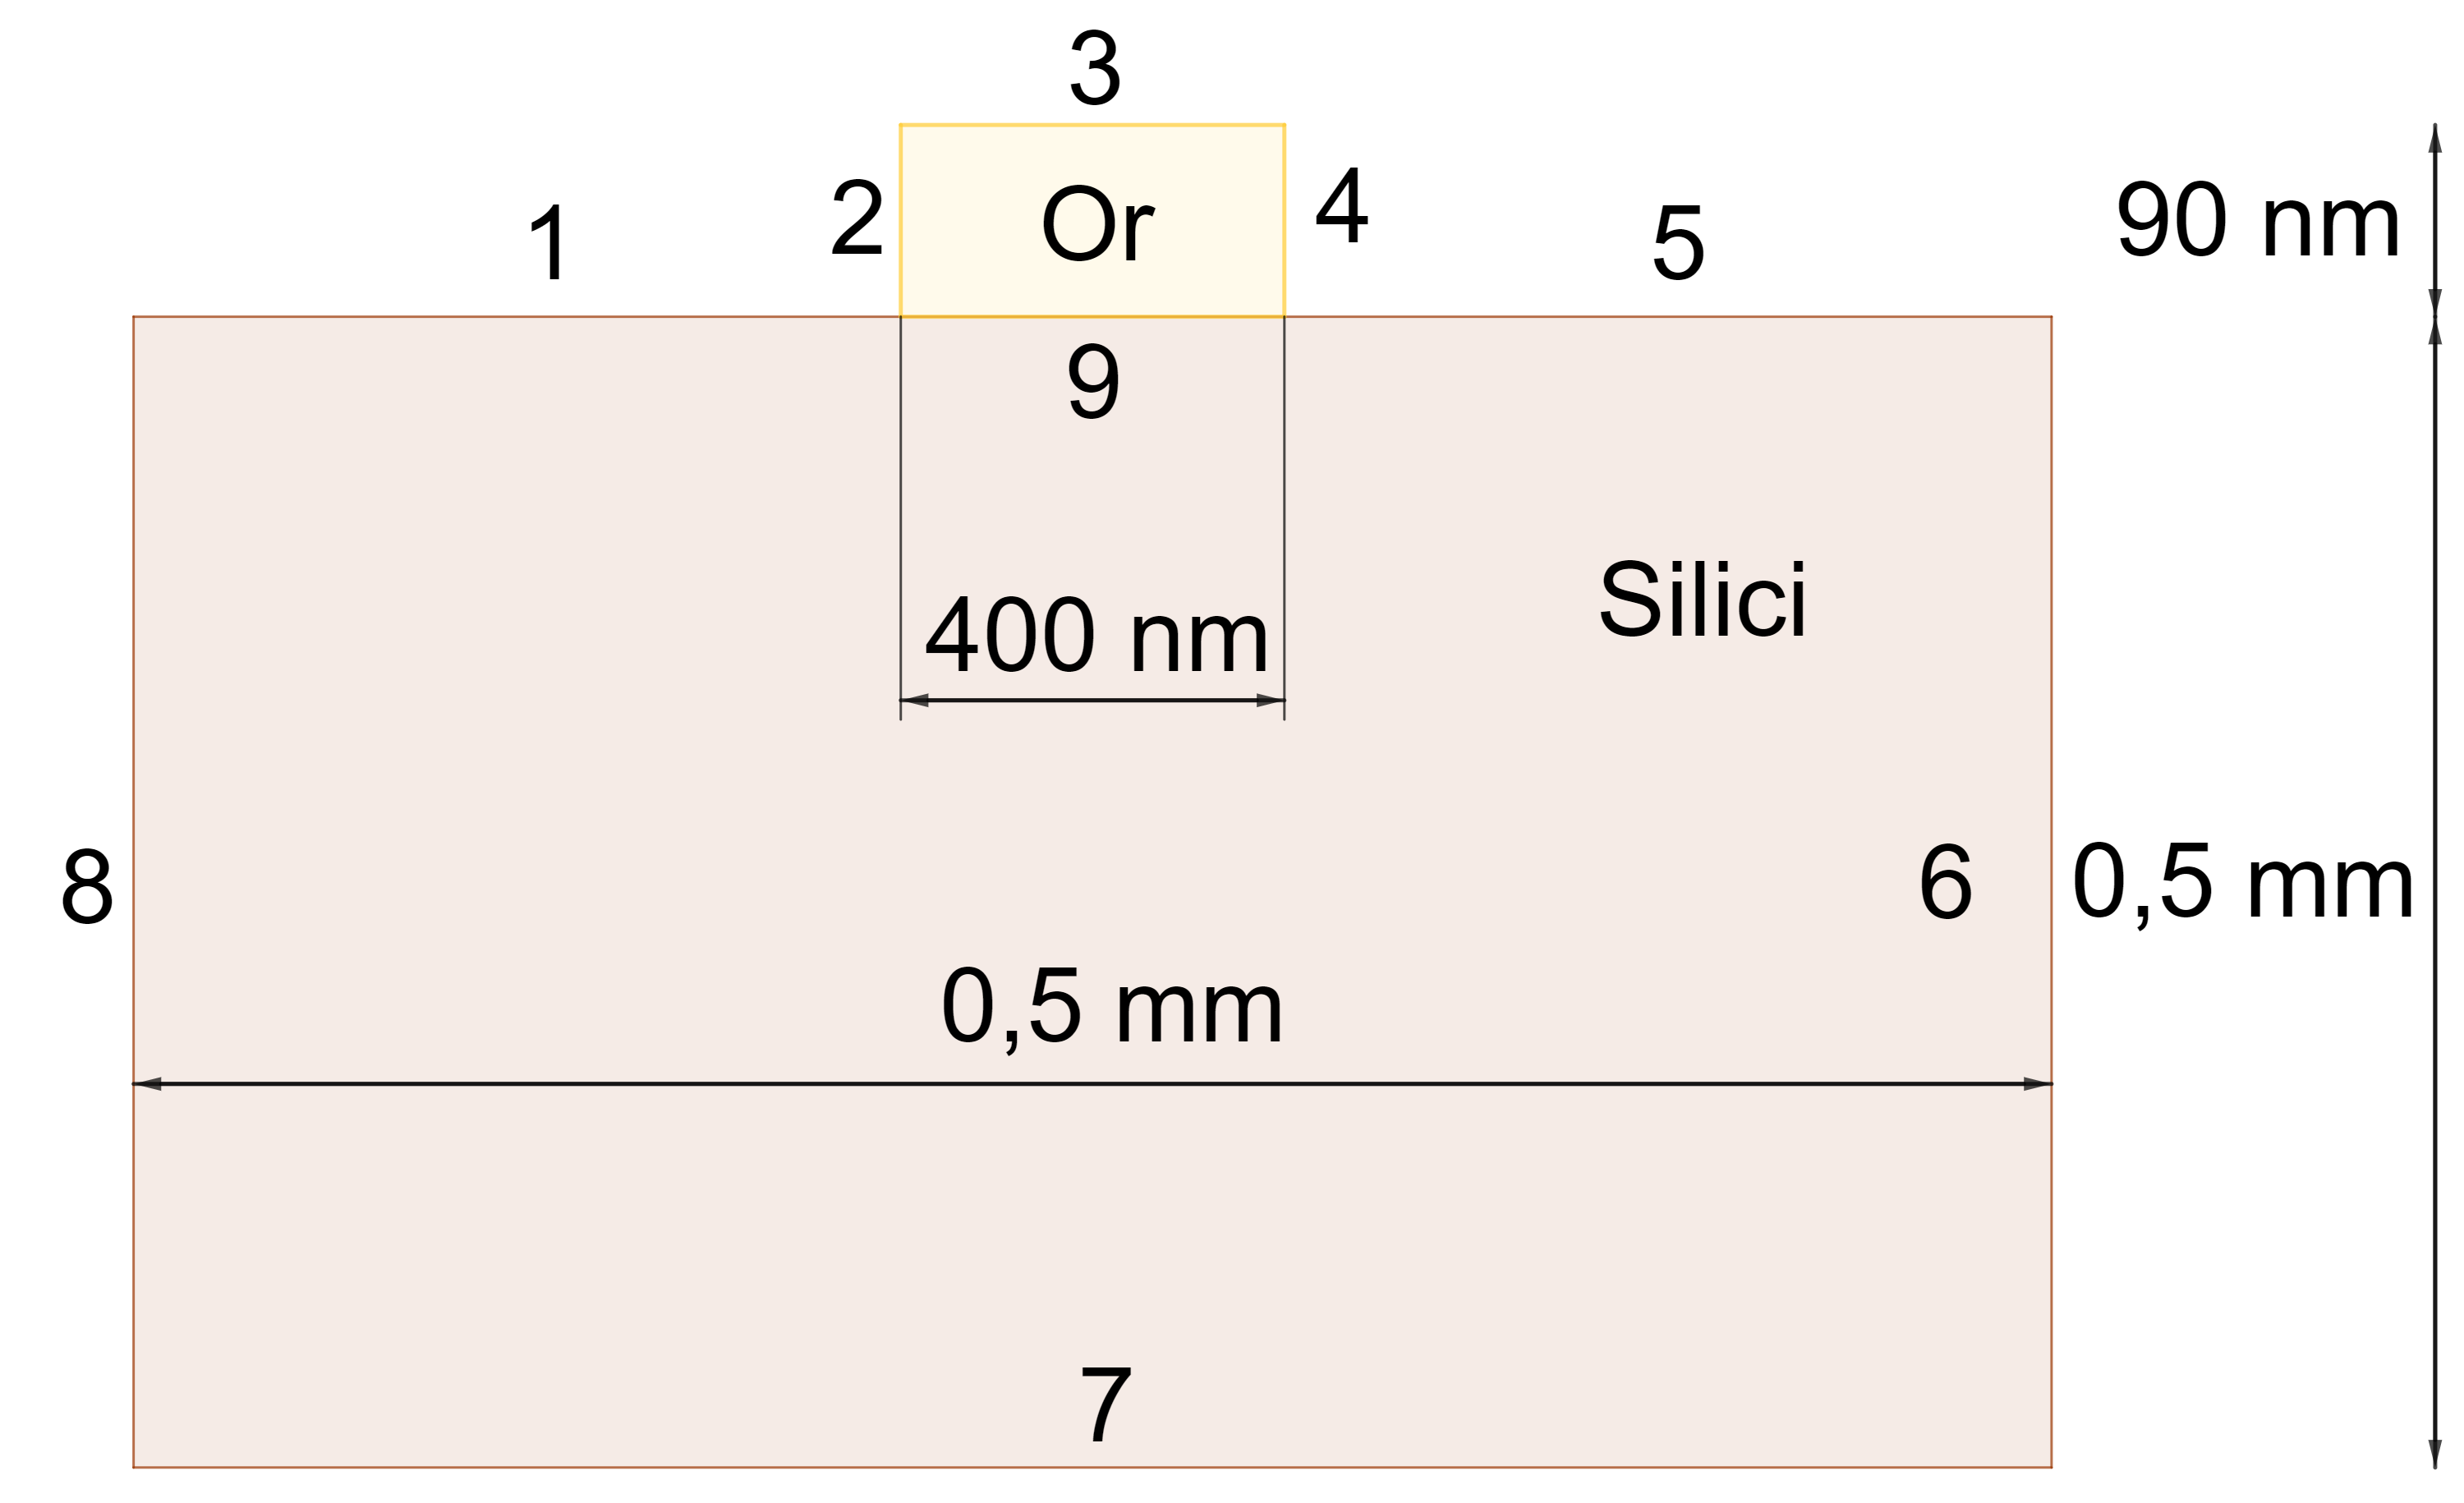
\includegraphics[scale=1]{../grafics/esquema/esquema.png}
\caption{Esquema no a escala de la segona simulaci\'{o}. Es representa el rectangle d'or sobre el rectangle de silici amb les dimensions preses per fer la simulaci\'{o}. Tamb\'{e} s'han numerat les parets del sistema per referir-nos a elles m\'{e}s f\`{a}cilment.}
\label{Fig:esquema2}
\end{center}
\end{figure}

Simularem nom\'{e}s dos rectangles: un ser\`{a} de silici i l'altre ser\`{a} d'or. La capa d'\`{o}xid es considerar\`{a} com a condici\'{o} de contorn a la frontera entre els dos rectangles. A l'article  \cite{torres2018emergence} es va realitzar tamb\'{e} aquesta simulaci\'{o} i aporta dades experimentals que farem servir per comparar-les amb els valors te\`{o}rics obtinguts mitjan\c{c}ant la nostra simulaci\'{o}.

Farem en aquest model tamb\'{e} una simulaci\'{o} per la llei de Fourier i una altra pel KCM. Aquesta segona consistir\`{a} a suposar la llei de Fourier sobre l'or i el model hidrodin\`{a}mic sobre el silici. Aquesta diferenciaci\'{o} est\`{a} justificada perqu\`{e} els portadors de calor en els dos medis s\'{o}n diferents. A l'or, que \'{e}s un metall ---i, per tant, conductor---, s\'{o}n els electrons els que porten la calor, mentre que al silici, que \'{e}s un semimetall a\"{i}llant, s\'{o}n els fonons els portadors. Pel comentat al marc te\`{o}ric, la llei de Fourier es pot aplicar a l'or, fins i tot a l'escala nanom\`{e}trica, ja que els electrons tenen un recorregut lliure mitj\`{a} molt m\'{e}s petit que les mides caracter\'{i}stiques del sistema i per tant els efectes no locals s\'{o}n gaireb\'{e} imperceptibles. Pel silici, en canvi, s\'{i} que s'ha d'utilitzar el model hidrodin\`{a}mic.

Comencem resolent el problema per la llei de Fourier. Considerem el nostre sistema a\"{i}llat t\`{e}rmicament i per tant posem sobre les parets 1, 2, 3, 4 i 5 de la Figura \ref{Fig:esquema2} la condici\'{o} de contorn \eqref{Equ.aillament}. Per altra banda, suposem que el substrat que estem simulant \'{e}s prou gran perqu\`{e} les parets 6, 7 i 8 ja estiguin a temperatura ambient. Per tant posem sobre elles la condici\'{o} de contorn $T=300$ K. Nom\'{e}s ens queda posar les condicions de contorn \eqref{Equ.continuitat} i \eqref{Equ.resistencia} sobre la paret 9.

Per simular l'escalfament de l'or per efecte Joule, hi afegim una font de calor uniforme $Q$ al rectangle superior. Anem posant valors de $Q$ cada cop m\'{e}s elevats fins que comencem a veure una difer\`{e}ncia considerable de temperatures entre les zones properes a la font i les m\'{e}s llunyanes que ens permeti estudiar el comportament del sistema.

En aquest punt passem a veure la mida que ha de tenir el substrat. Idealment el substrat seria molt gran, per\`{o} el m\`{e}tode d'elements finits t\'{e} un l\'{i}mit sobre la quantitat de c\`{a}lculs que pot fer en un espai raonable de temps. Per\`{o} si fem el substrat massa petit, els efectes de contorn de les parets 6, 7 i 8 afectarien directament la temperatura de la part del substrat que est\`{a} tocant la font, reduint-la. Per aix\`{o} busquem la mida \`{o}ptima, que ser\`{a} la m\'{i}nima mida per la qual la temperatura m\`{a}xima del substrat ---assolida al costat de la font--- sigui gaireb\'{e} la mateixa que la que tindria si el substrat fos infinit. Per trobar-la, comencem amb una mida massa petita i l'anem fent m\'{e}s gran, fins que la temperatura m\`{a}xima deixi d'incrementar-se.

Un altre par\`{a}metre que hem de determinar per tal de fer b\'{e} l'experiment i aconseguir uns resultats acurats \'{e}s la mida i forma de la malla dels elements finits. Per resoldre el sistema per la llei de Fourier no hi ha cap problema: nom\'{e}s cal una malla m\'{e}s fina al voltant de l'or, on tingui una separaci\'{o} entre nodes de l'ordre dels nan\`{o}metres, ja que a aquesta zona les variacions de les magnituds s\'{o}n molt m\'{e}s grans que a la resta del substrat, on les magnituds s\'{o}n molt uniformes. Per\`{o} pel model hidrodin\`{a}mic tenim el problema de les cantonades. A l'equaci\'{o} \eqref{Equ.estacionari} hi apareix el laplaci\`{a}, que involucra segones derivades i aquest terme causa que les derivades al voltant d'angles rectes es facin infinites. Per tant a un entorn petit dels extrems de la paret 9, el m\`{e}tode d'elements finits no convergir\`{a}. Per tal de reduir aquesta zona de no converg\`{e}ncia, fem molt m\'{e}s fina encara la malla a la barra d'or i a les regions properes. Lluny d'aquesta regi\'{o} la temperatura varia molt poc i es poden separar els nodes, alleugerant la quantitat de c\`{a}lculs necess\`{a}ria per resoldre el sistema. Si la malla no \'{e}s prou fina, es veuen punts angulosos al diagrama de temperatures que indiquen que a aquella zona no s\'{o}n correctes els c\`{a}lculs. Considerem una malla prou fina quan aquests punts angulosos desapareixen i tenim una distribuci\'{o} llisa de temperatures.

Despr\'{e}s ajustem un altre cop el valor de $Q$ perqu\`{e} la temperatura que assoleix la barra sigui la utilitzada a l'article \cite{torres2018emergence}. Finalment, quan ja ho tenim tot constru\"{i}t, representem a una gr\`{a}fica la temperatura de la part superior del substrat al voltant de la barra d'or, per\`{o} a la posici\'{o} de la barra, representem la temperatura de la part de dalt de la barra. Aix\`{o} respon a dos motius: primer, l'experiment realitzat a \cite{ziabari2017non} mesura la temperatura de la part superior del sistema i segon, l'objectiu \'{e}s estudiar el refredament de components electr\`{o}nics posats sobre un substrat. Per tant ens interessa saber quant s'escalfa i quina temperatura assoleix el conductor.

\subsection{Resultats i an\`{a}lisi de dades}

\begin{figure}[ht!]
\begin{center}
\includegraphics[scale=0.8]{../grafics/estacionari/experimentals.png}
\caption{Gr\`{a}fica de la temperatura a la part superior del substrat i de l'or respecte la posici\'{o} $x$ segons Fourier (morat), segons KCM (blau) i segons Fourier amb la conductivitat efectiva (verd). S'han representat tamb\'{e} els punts experimentals (taronja) obtinguts de l'article \cite{torres2018emergence}.}
\label{Fig:Orexp}
\end{center}
\end{figure}

A la Figura \ref{Fig:Orexp} podem trobar una gr\`{a}fica de la temperatura a la part superior del sistema al voltant de la barra d'or. S'ha triat una conductivitat t\`{e}rmica del substrat de $124 $ W/(m$\cdot$K) i una longitud no local de $160$ nm. La barra d'or t\'{e} $400$ nm d'amplada i $90$ nm d'al\c{c}ada i la resist\`{e}ncia t\`{e}rmica de la frontera entre ambd\'{o}s materials \'{e}s de $25$ nKm$^2$/W. Els par\`{a}metres del silici s\'{o}n diferents dels de l'apartat anterior perqu\`{e} corresponen al silici dopat amb \`{a}toms de bor, que \'{e}s el que s'ha utilitzat a l'article \cite{torres2018emergence}, d'on extraiem les dades experimentals. Despr\'{e}s d'haver determinat les mides que ha de tenir el substrat i la magnitud de la font t\`{e}rmica, hem decidit un substrat quadrat de costat $0,5$ mm i una font de densitat de calor $Q=1,02\cdot10^{16}$ W/m$^3$. A les parets externes (esquerra, dreta i inferior) del substrat del silici s'imposa una temperatura de $300$ K. Tant amb Fourier com amb el KCM es pot apreciar un salt de temperatura justament on comen\c{c}a l'or. Aquesta discontinu\"{i}tat est\`{a} justificada perqu\`{e} estem prenent la temperatura del substrat i de sobte comencem a prendre la temperatura de la barra, que s\'{o}n objectes diferents. Entre aquests objectes hi ha una frontera sobre la qual hem imposat les condicions de contorn de continu\"{i}tat de la component normal del flux \eqref{Equ.continuitat} i de discontinu\"{i}tat de temperatures \eqref{Equ.resistencia}. Aquesta \'{u}ltima \'{e}s deguda a la resist\`{e}ncia t\`{e}rmica de frontera i \'{e}s la que provoca aquest salt  de temperatura.

A la mateixa gr\`{a}fica es pot apreciar una disminuci\'{o} de la temperatura a les vores de l'or, fins i tot per sota de la temperatura de 300 K que hem fixat a les parets laterals i inferior del substrat. Nom\'{e}s succeeix amb el model hidrodin\`{a}mic i de fet \'{e}s al voltant dels angles rectes formats per la uni\'{o} de la barra i el substrat, on hav\'{i}em dit que no pod\'{i}em garantir que la soluci\'{o} convergeixi. A m\'{e}s, no hi ha cap fenomen f\'{i}sic que expliqui aquesta caiguda de temperatura ni evid\`{e}ncia experimental que li doni suport. Apart, a mesura que s'anava refinant la malla, aquesta baixada de temperatura s'anava atenuant. Aquests fets suggereixen que el motiu d'aquest fenomen observat no \'{e}s f\'{i}sic, sin\'{o} que resideix en una precisi\'{o} limitada del m\`{e}tode dels elements finits. De totes maneres, fora de la regi\'{o} que envolta les cantonades, els c\`{a}lculs fets s\'{o}n perfectament v\`{a}lids.

Observem tamb\'{e} que les prediccions de Fourier i del model KCM s\'{o}n diferents. A l'hora d'estimar la temperatura del silici, a les cues, coincideixen, per\`{o} difereixen en la temperatura de l'or. La llei de Fourier calcula una temperatura a la barra d'or de 331,0 K, que \'{e}s inferior a l'esperada pel model hidrodin\`{a}mic, la qual temperatura \'{e}s 333,1 K. Aquesta difer\`{e}ncia s'explica pels efectes no locals: la mida de la barra d'or \'{e}s de l'ordre del recorregut lliure mitj\`{a} dels fonons que porten la calor al silici. Per tant aquests efectes s\'{o}n perceptibles i fan que la calor es transmeti menys eficientment, ja que recordem que el terme de no localitat \'{e}s una mena de viscositat que arrossega el lliscament amb les parets disminuint el flux de calor. Per aquest motiu, el model KCM prediu un refredament m\'{e}s pobre de l'or, resultant en un increment de la seva temperatura.

Aquestes difer\`{e}ncies entre els dos models ja no es poden esquivar fent \'{u}s d'una conductivitat t\`{e}rmica efectiva redu\"{i}da a la llei de Fourier. Al mateix gr\`{a}fic es veu que si s'utilitza una conductivitat efectiva tal que la temperatura de l'or coincideixi per ambd\'{o}s models, el que s'est\`{a} fent \'{e}s pujar la temperatura predita per Fourier a tot el sistema i per tant les cues de la gr\`{a}fica deixen de coincidir. A la simulaci\'{o} de la l\`{a}mina fina encara amb una conductivitat t\`{e}rmica efectiva pod\'{i}em explicar alhora la distribuci\'{o} de temperatures i la calor total transmesa ---tot i que no pogu\'{e}ssim explicar el perfil del flux de calor---. Per\`{o} en el cas de la barra d'or no podem ni tan sols explicar la distribuci\'{o} de temperatures sencera amb la llei de Fourier i una conductivitat efectiva.

\begin{figure}[ht!]
\begin{center}
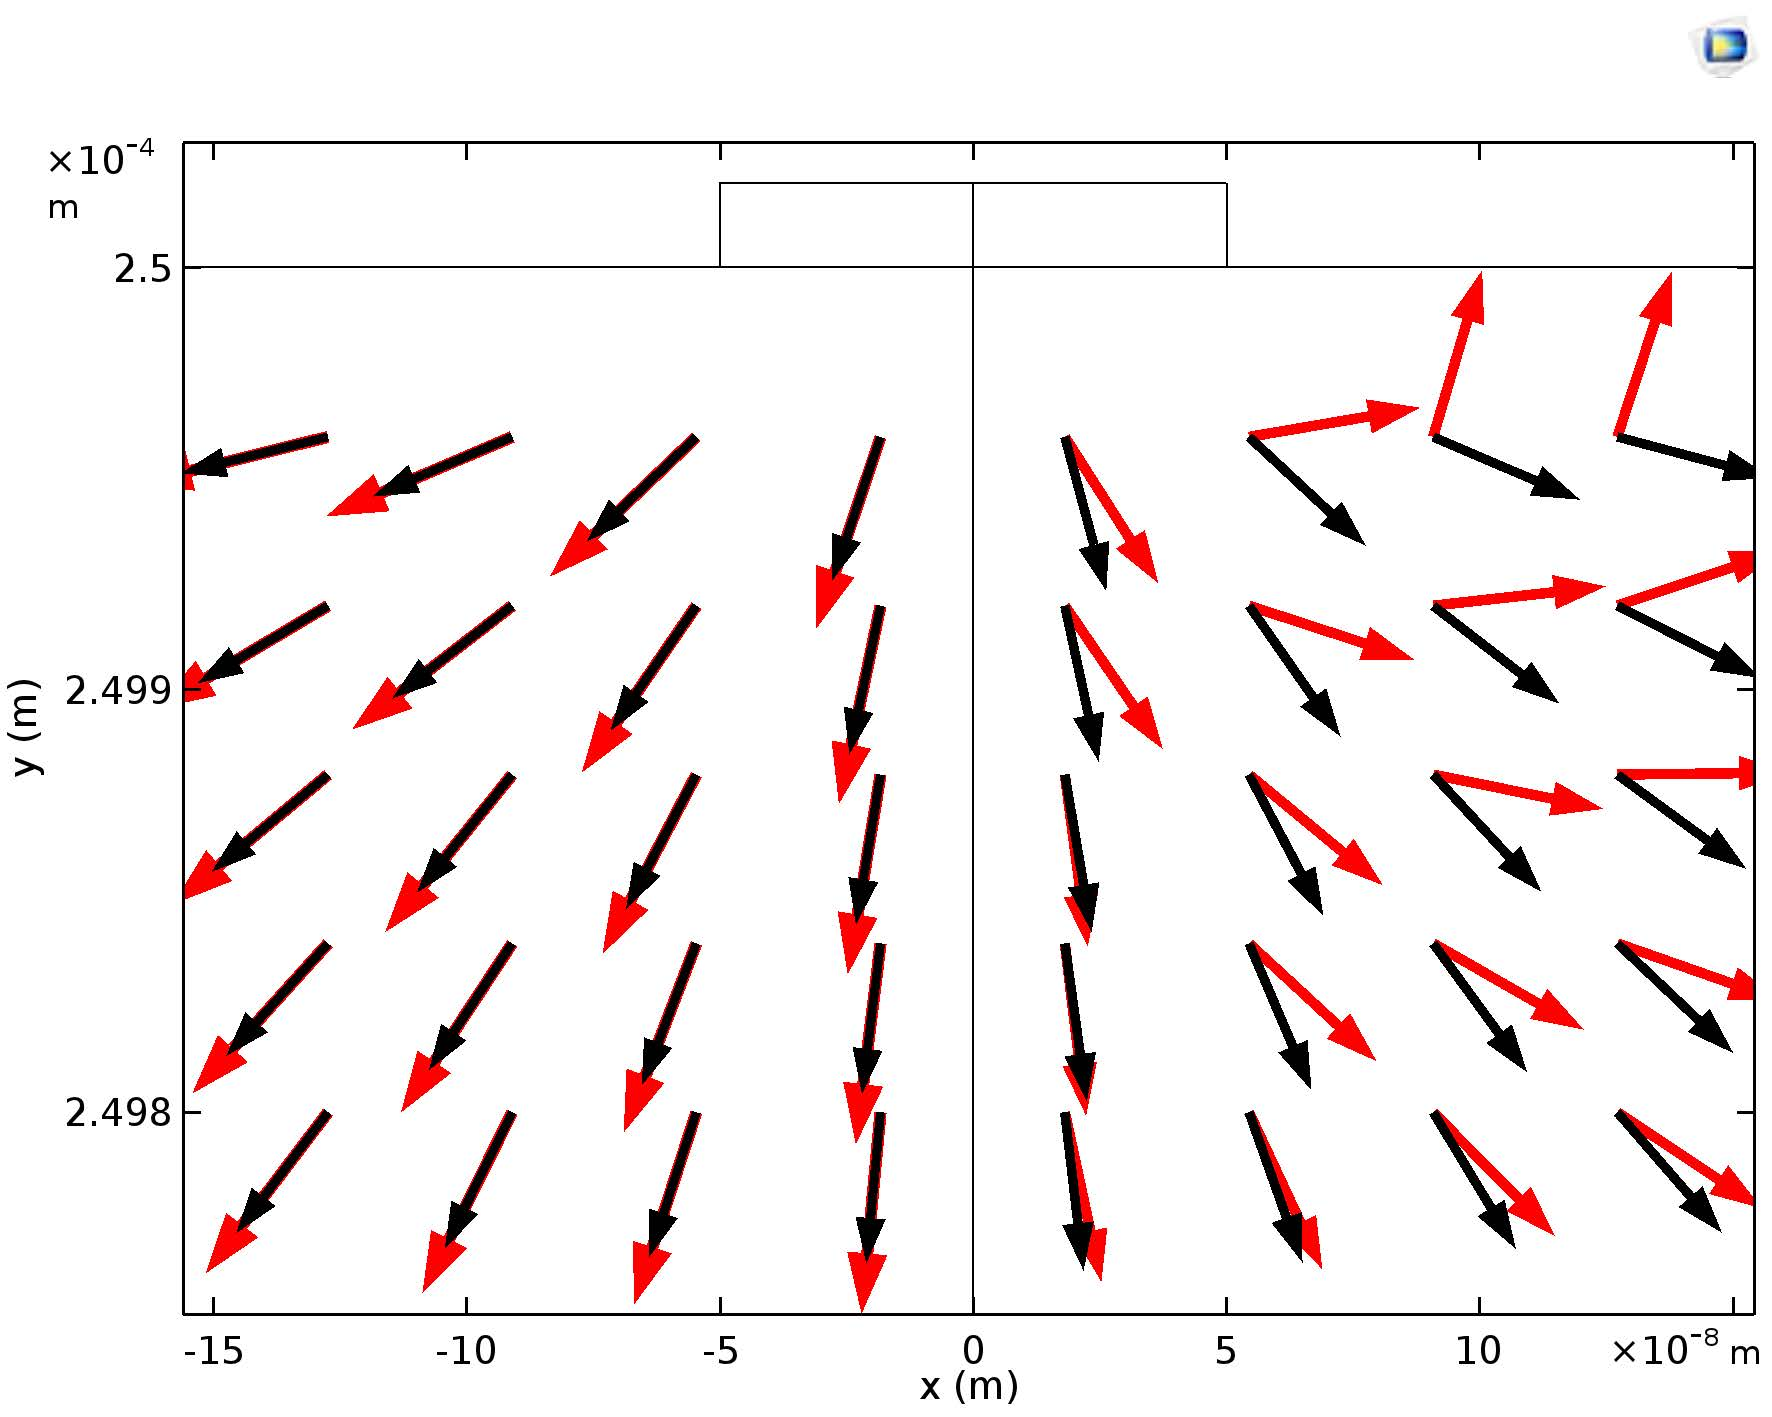
\includegraphics[scale=0.7]{../grafics/estacionari/temperatura-flux.jpg}
\caption{Diagrama de fletxes del flux de calor (negre) i el gradient de temperatures (vermell). A la meitat esquerra del dibuix es representen els vectors obtinguts de la llei de Fourier i a la meitat dreta es representen els del model hidrodin\`{a}mic. Nom\'{e}s volem comparar les direccions d'aquests vectors, no la seva intensitat, i per aix\`{o} s'han representat normalitzats. Les fletxes del gradient de temperatures es representen m\'{e}s grans per distingir-les m\'{e}s clarament d'aquelles del flux de calor, sobre tot quan s\'{o}n paral\textperiodcentered leles.}
\label{Fig:Fletxes}
\end{center}
\end{figure}

A la Figura \ref{Fig:Fletxes} es comparen el flux de calor i el gradient de temperatures segons la llei de Fourier i el model hidrodin\`{a}mic. Podem observar com a la part de Fourier aquests dos vectors sempre s\'{o}n paral\textperiodcentered lels, com estipula la llei de Fourier. A la part del KCM, en canvi, no s\'{o}n molt paral\textperiodcentered lels. De totes maneres, just sota l'escalfador s\'{i} que s\'{o}n paral\textperiodcentered lels, mentre que a la part m\'{e}s dreta arriben a ser fins i tot perpendiculars. Aix\`{o} s'explica per la conservaci\'{o} de moment lineal dels fonons. Els fonons surten de l'escalfador amb direcci\'{o} vertical i sentit cap avall. Si un fon\'{o} no col\textperiodcentered lideix amb cap altre fon\'{o}, continuar\`{a} el seu recorregut seguint un moviment rectilini uniforme. Ser\`{a} nom\'{e}s quan col\textperiodcentered lideixi amb un altre fon\'{o} que podr\`{a} canviar de direcci\'{o} i propagar-se en direcci\'{o} horitzontal. Llavors si el recorregut lliure mitj\`{a} \'{e}s molt m\'{e}s petit que les longituds caracter\'{i}stiques de la geometria del sistema, els fonons patiran tantes col\textperiodcentered lisions que la conservaci\'{o} de moment lineal gaireb\'{e} no tindr\`{a} rellev\`{a}ncia i els fonons tendiran a distribuir-se i moure's segons el gradient de temperatures. Per\`{o} si les dimensions s\'{o}n de l'ordre de $\ell$, els fonons tendiran a mantenir el seu moment, que ser\`{a} vertical, i la transmissi\'{o} de la calor en la direcci\'{o} horitzontal ser\`{a} m\'{e}s petita del que li correspondria. Aquest fet \'{e}s el causant de la discrep\`{a}ncia entre la direcci\'{o} del flux i el gradient de temperatures a la zona dreta del diagrama, mentre que sota la barra aquests dos vectors s\'{o}n bastant paral\textperiodcentered lels, ja que en la direcci\'{o} vertical s\'{i} que hi ha prou fonons viatjant.

Tornant a la Figura \ref{Fig:Orexp}, si observem les dades experimentals, veiem que a les cues s'adeq\"{u}en b\'{e} a les cues del model KCM. A m\'{e}s, la temperatura de l'or obtinguda experimentalment coincideix amb el model KCM. Ja hem vist que per aquesta configuraci\'{o} el model de Fourier i el KCM s\'{o}n incompatibles. Per aquestes raons \'{u}nicament el model KCM ha estat capa\c{c} d'explicar les dades experimentals i ser\`{a} el que fem servir per tractar de reduir la temperatura de l'or.

\section{Barra d'or sobre un substrat escalfat peri\`{o}dicament}

\subsection{Metodologia}

Per \'{u}ltim, volem fer algun invent tecnol\`{o}gic per disminuir la temperatura de l'or de la simulaci\'{o} anterior. Per all\`{o} hi afegim una font de calor de $14$ nm de profunditat a la part superior del substrat de silici. Aquesta font de calor pret\'{e}n reproduir un escalfament peri\`{o}dic per un l\`{a}ser monocrom\`{a}tic que t\'{e} una freq\"{u}\`{e}ncia $\nu=200$ MHz i que t\'{e} una profunditat \`{o}ptica de $14$ nm. L'objectiu de posar aquesta font \'{e}s reduir la $\ell$ intr\'{i}nseca del silici a una $\ell$ efectiva de $14$ nm, amb el qual reduir els efectes no locals i que la predicci\'{o} del model hidrodin\`{a}mic s'acosti a la de la llei de Fourier, produint-se un descens de la temperatura de l'or.

Per modelitzar el l\`{a}ser, simulem una font de calor que decau amb la dist\`{a}ncia $d$ amb la paret superior segons un factor $e^{-(d/14\text{nm})^2}$, de manera que la longitud caracter\'{i}stica de la font i, per tant, la longitud que podem considerar de la font, \'{e}s $14$ nm. El decreixement \'{e}s degut a l'absorci\'{o} progressiva dels fotons per part dels electrons del substrat i \'{e}s exponencial segons dicta la llei de Beer-Lambert \cite{lambert1760jh}, que afirma que el decreixement en la intensitat de la llum absorbida \'{e}s proporcional a la intensitat.

A la zona on hi ha la font, com que \'{e}s tan prima i la seva intensitat decau tan r\`{a}pidament, s'ha de refinar la malla del m\`{e}tode d'elements finits, perqu\`{e} si els elements s\'{o}n massa grans, el valor de $Q$ varia molt dins l'element. Recordem que el substrat \'{e}s molt gran respecte a l'or. Per tant necessitar\'{i}em una quantitat excessiva d'elements per cobrir tota la part superior del substrat. Per\`{o}, com que nom\'{e}s ens interessa la temperatura de l'or i els seus voltants, n'hi ha prou amb posar la font del l\`{a}ser a una regi\'{o} petita a prop de l'or. Concretament, multipliquem $Q$ per un factor $e^{-(x/5\mu\text{m})^2}$, on $x$ \'{e}s la coordenada horitzontal amb origen al centre del sistema. D'aquesta manera, podem reduir molt el nombre d'elements necessaris lluny de l'or, alleugerant c\`{a}lculs innecessaris.

Amb tot el que hem dit, obtenim l'expressi\'{o} de la font de calor:
\[Q=Q_{\text{m\`{a}x}}e^{-(d/14\text{nm})^2}e^{-(x/5\mu\text{m})^2}\sin^2(2\pi\nu t).\]

El quadrat del sinus sorgeix perqu\`{e} l'amplitud de l'ona del l\`{a}ser oscil\textperiodcentered la segons el sinus i per tant la pot\`{e}ncia de l'ona porta un quadrat, fent que la freq\"{u}\`{e}ncia de la calor sigui $2\nu$.

Si volgu\'{e}ssim calcular la soluci\'{o} dependent del temps, obtindr\'{i}em un estat transitori en el que la temperatura aniria augmentant fins assolir un estat peri\`{o}dic en qu\`{e} oscil\textperiodcentered laria amb la freq\"{u}\`{e}ncia de la font. De totes maneres, aquestes oscil\textperiodcentered lacions no serien molt grans, ja que no posarem una pot\`{e}ncia molt elevada. Volem principalment estudiar la temperatura mitjana de la barra d'or per veure que el l\`{a}ser provoca una reducci\'{o} de la temperatura. Per aquesta ra\'{o} en tenim prou amb calcular l'estat estacionari, que constru\"{i}m amb una font t\`{e}rmica que doni una calor igual a la mitjana temporal del l\`{a}ser:
\[Q=\frac 1 2Q_{\text{m\`{a}x}}e^{-(d/14\text{nm})^2}e^{-(x/5\mu\text{m})^2}.\]

Com a valor de $Q_{\text{m\`{a}x}}$ hem d'agafar un que sigui suficient per ser capa\c{c} d'afectar la longitud no local efectiva. A l'article \cite{beardo2020phonon} es simula una situaci\'{o} semblant: una l\`{a}mina prima d'or sobre un substrat de germani escalfada peri\`{o}dicament
per un l\`{a}ser. En aquesta simulaci\'{o} s'utilitza un $Q_{\text{m\`{a}x}}$ tal que la temperatura de la part superior del substrat ---sense l'escalfador met\`{a}l\textperiodcentered lic--- s'eleva 3 K per sobre de la temperatura de refer\`{e}ncia i aquesta font de calor \'{e}s suficient per reduir la longitud no local efectiva. Per tant anirem provant diferents $Q_{\text{m\`{a}x}}$ fins aconseguir aquest increment de 3 K. Cal remarcar que a aquest article el substrat \'{e}s de germani, no de silici. Tot i aix\'{i}, tots dos elements s\'{o}n semiconductors del mateix grup i per tant s'espera que es comportin d'igual manera. De totes maneres, per acabar de confirmar el descens de temperatura de l'escalfador, hauria de comprovar-se experimentalment. A aquest treball, per\`{o} nom\'{e}s ho comprovarem te\`{o}ricament mitjan\c{c}ant la simulaci\'{o} abans exposada. De totes maneres, \'{e}s esperable que la $\ell$ efectiva prengui aquest valor perqu\`{e} aquest fenomen s'ha observat tamb\'{e} en altres experiments, com l'exposat a l'article \cite{beardo2021general}, on es posen escalfadors met\`{a}l\textperiodcentered lics sobre un substrat de silici i s'ha provat que la $\ell$ efectiva \'{e}s la meitat de la dist\`{a}ncia entre escalfadors.

\subsection{Resultats i an\`{a}lisi de dades}

\begin{figure}[ht!]
\begin{center}
\begin{subfigure}{.49\textwidth}
\caption{}
\label{Fig:TeoriquesEst}
\includegraphics[scale=0.39]{../grafics/estacionari/teoriques.png}
\end{subfigure}
\begin{subfigure}{.49\textwidth}
\caption{}
\label{Fig:TeoriquesPer}
\includegraphics[scale=0.39]{../grafics/periodic/teoriques.png}
\end{subfigure}
\caption{Gr\`{a}fiques de la temperatura a la part superior del substrat i de l'or respecte la posici\'{o} $x$ segons Fourier (morat) i segons KCM (verd). S'ha representat sense el l\`{a}ser a la gr\`{a}fica (a) i amb el l\`{a}ser a la gr\`{a}fica (b).}
\label{Fig:Teoriques}
\end{center}
\end{figure}

A la Figura \ref{Fig:Teoriques} hi ha dues gr\`{a}fiques comparant la temperatura del sistema sense i amb el l\`{a}ser escalfant la part superior del substrat. Hem pres els mateixos par\`{a}metres que a l'apartat anterior, per\`{o} reduint la resist\`{e}ncia t\`{e}rmica a 5 nKm$^2$/W, l'amplada de la barra a $200$ nm i la seva al\c{c}ada a $45$ nm. Per adaptar la font de calor de la barra a aquests canvis, l'hem substitu\"{i}da per $2,3\cdot10^{16}$ W/m$^3$. Aquests canvis de par\`{a}metres s'han fet perqu\`{e} les difer\`{e}ncies entre els models siguin m\'{e}s accentuades i es puguin apreciar millor. A part, seguint el m\`{e}tode exposat a la metodologia, s'ha vist que la calor del l\`{a}ser ha de ser $Q_{\text{m\`{a}x}}=3,7\cdot10^{15}$ W/m$^3$. A les gr\`{a}fiques es pot veure que la temperatura del silici augmenta, com \'{e}s esperable. Tamb\'{e} augmenta la temperatura de l'or segons la predicci\'{o} de Fourier: passa de 320,1 K a 321,2 K. Aquests augments de temperatures s\'{o}n bastant intu\"{i}tius, per\`{o} segons el model hidrodin\`{a}mic, la temperatura de l'or ha disminu\"{i}t des dels 326,9 K als 323,6 K. Aquesta disminuci\'{o} de temperatura s'ha aconseguit \'{u}nicament afegint-hi la calor del l\`{a}ser, el qual pot resultar paradoxal. Tanmateix, t\'{e} la seva explicaci\'{o}: en escalfar una fina capa de 14 nm del substrat de silici, hem fet que la longitud caracter\'{i}stica del sistema sigui de 14 nm i amb aix\`{o}, al model KCM, s'ha de prendre una $\ell$ efectiva de 14 nm. Aix\`{o} provoca que el terme visc\'{o}s de l'equaci\'{o} hidrodin\`{a}mica sigui molt m\'{e}s petit incrementant el flux de calor i refredant m\'{e}s eficientment la barra.

Per tant el l\`{a}ser provoca dos efectes contraris que modifiquen la temperatura de l'escalfador. Per una banda, el l\`{a}ser que escalfa el substrat inevitablement ha d'escalfar tamb\'{e} l'or ---com s'aprecia al model de Fourier--- i per altra banda, redueix la longitud no local efectiva incrementant el flux de calor al model KCM i aix\'{i} baixant la temperatura de la barra d'or. A la nostra simulaci\'{o} hem aconseguit que d'aquests dos efectes tingui m\'{e}s pes el segon mencionat, obtenint un descens a la temperatura del metall. Ha estat possible gr\`{a}cies a que la dist\`{a}ncia de penetraci\'{o} del l\`{a}ser era prou petita per reduir molt la longitud no local efectiva i a un equilibri molt fi a la pot\`{e}ncia del l\`{a}ser: si hagu\'{e}s tingut poca pot\`{e}ncia, no hauria estat capa\c{c} de modificar la $\ell$ efectiva i si hagu\'{e}s tingut massa pot\`{e}ncia, l'escalfament de l'or degut al l\`{a}ser hauria estat m\'{e}s alt que el refredament degut a baixar la $\ell$ efectiva.

\begin{figure}[ht!]
\begin{center}
\includegraphics[scale=0.7]{../grafics/periodic/diferencies-or.png}
\caption{Gr\`{a}fica de la difer\`{e}ncia de temperatures de la barra d'or entre la llei de Fourier i el model hidrodin\`{a}mic per diverses amplades de la barra, sempre mantenint la mateixa ra\'{o} entre l'al\c{c}ada i l'amplada de $90:400$. En blau es representen les difer\`{e}ncies produ\"{i}des sense el l\`{a}ser i en vermell, amb el l\`{a}ser.}
\label{Fig:Diferencies}
\end{center}
\end{figure}

Tamb\'{e} s'ha mesurat la temperatura de la barra d'or segons la llei de Fourier i segons el model hidrodin\`{a}mic i s'han representat les difer\`{e}ncies a la Figura \ref{Fig:Diferencies}. S'ha anat variant l'amplada i l'al\c{c}ada de la barra sempre mantenint fixa la seva ra\'{o}. A m\'{e}s, la densitat horitzontal de calor de la font de l'or s'ha mantingut fixa, \'{e}s a dir, a doble d'amplada de la barra li corresponia el doble d'al\c{c}ada i per tant la meitat de densitat de calor generat, ja que l'al\c{c}ada era doble. Al gr\`{a}fic es veu clarament com, sense el l\`{a}ser, quan es fa petita la mida de la barra, les difer\`{e}ncies s'accentuen, cosa explicable perqu\`{e} ens apropem a la mida del recorregut lliure mitj\`{a} dels fonons, fent que els efectes no locals dominin. En canvi, amb el l\`{a}ser es mant\'{e} sempre una difer\`{e}ncia petita i bastant constant, que t\'{e} explicaci\'{o} en la disminuci\'{o} de la dist\`{a}ncia no local efectiva, que acaba sent bastant m\'{e}s petita que l'amplada de la barra i per tant no s\'{o}n tan pronunciats els efectes de disminuir la seva amplada.

En conclusi\'{o}, hem aconseguit l'objectiu que esper\`{a}vem: baixar la temperatura de l'escalfador met\`{a}l\textperiodcentered lic. Aquesta reducci\'{o} de temperatura \'{e}s m\'{e}s not\`{o}ria com m\'{e}s petita \'{e}s la mida de la barra d'or. Fixem-nos que amb aquest m\`{e}tode mai no podrem abaixar la temperatura de l'escalfador per sota de la temperatura donada per la llei de Fourier. Aix\`{o} \'{e}s aix\'{i} perqu\`{e} ens estem basant a reduir la $\ell$ efectiva. Per tant el punt l\'{i}mit seria l'hipot\`{e}tic cas en qu\`{e} $\ell=0$. En aquesta situaci\'{o} recuperar\'{i}em la llei de Fourier. Per aix\`{o}, la m\'{i}nima temperatura que podr\'{i}em assolir seria la predita per Fourier. Tornant a les nostres dades (amplada de la barra de 200 nm), hem passat de 326,9 K a 323,6 K, sent la m\'{i}nima temperatura que pod\'{i}em assolir de 320,1 K. Podem dir que la reducci\'{o} ha estat prou satisfact\`{o}ria. Aquest fenomen s'ha aconseguit simular, per\`{o} encara faltaria comprovar-lo experimentalment, ja que hem canviat manualment el valor de la $\ell$ del silici per un valor efectiu. Seria necessari principalment comprovar experimentalment que efectivament en aquest cas concret, la longitud no local $\ell$ pren aquest valor efectiu.

\section{Conclusions}

Hem posat a prova la llei de Fourier a la nanoscala. Aquesta \'{e}s la llei cl\`{a}ssica que governa la conducci\'{o} de la calor i que s'utilitza gaireb\'{e} sempre. Per aquest fi hem utilitzat primerament un sistema molt simple: una fina l\`{a}mina de silici. Hem vist que les dades experimentals implicaven una reducci\'{o} del flux de la calor que travessava la l\`{a}mina. Per explicar aquests resultats, hem utilitzat la llei de Fourier amb una conductivitat t\`{e}rmica efectiva i hem vist que pot compatibilitzar el gradient de temperatures amb la reducci\'{o} de la calor transmesa, per\`{o} te el problema que la conductivitat efectiva no \'{e}s una magnitud realment f\'{i}sica. Per aix\`{o} hem proposat un nou model: el model cin\`{e}tic col\textperiodcentered lectiu, obtingut fent aproximacions a partir de l'equaci\'{o} del transport de Boltzmann. Aquest model \'{e}s m\'{e}s general que la llei de Fourier en tenir en compte m\'{e}s termes a les seves equacions. Quan es treballa amb sistemes prou grans, es recupera la llei de Fourier, ja que aquests nous termes es tornen menyspreables. Aquest nou model s\'{i} que ha estat capa\c{c} d'explicar f\'{i}sicament la disminuci\'{o} del flux de calor.

Despr\'{e}s hem volgut dissenyar un m\`{e}tode que refred\'{e}s els conductors dels aparells electr\`{o}nics. Per aix\`{o} primer hem simulat una barra met\`{a}l\textperiodcentered lica d'or que s'escalfa per efecte Joule sobre un substrat de silici. Amb aquesta simulaci\'{o} hem ent\`{e}s com es transporta la calor en aquesta situaci\'{o}. El model hidrodin\`{a}mic que hem proposat abans predeia que el metall s'escalfava m\'{e}s i assolia una temperatura superior que la llei de Fourier. Hem comparat les temperatures d'ambd\'{o}s models amb temperatures obtingudes experimentalment i hem tornat a veure que s'adapten al model hidrodin\`{a}mic i que no es poden explicar amb la llei de Fourier. En aquest cas, ja ni tan sols s'han pogut explicar amb una conductivitat t\`{e}rmica efectiva per la llei de Fourier. Per tant, definitivament, hem d'utilitzar el model hidrodin\`{a}mic per obtenir un m\`{e}tode de refredar el conductor. A m\'{e}s aquesta necessitat de refredament es torna m\'{e}s necess\`{a}ria degut a que la temperatura real que assoleix el conductor \'{e}s m\'{e}s alta del que pod\'{i}em esperar utilitzant l'equaci\'{o} cl\`{a}ssica de conducci\'{o} de la calor (la llei de Fourier).

Sabem que si hi ha una longitud caracter\'{i}stica del sistema m\'{e}s petita que la longitud no local, aquesta \'{u}ltima pren un valor efectiu igual a aquella longitud caracter\'{i}stica. Per tant, escalfant amb un l\`{a}ser una zona d'amplada molt petita, redu\"{i}m la longitud no local efectiva i, amb ella, els efectes no locals que redueixen el flux de calor, resultant en una reducci\'{o} de la temperatura del conductor. Hem simulat aquesta configuraci\'{o} i segons la llei de Fourier la temperatura s'ha incrementat, per\`{o} segons el model hidrodin\`{a}mic ha disminu\"{i}t. De totes maneres, hav\'{i}em comprovat que nom\'{e}s el model hidrodin\`{a}mic era v\`{a}lid a les escales en qu\`{e} estem treballant, de manera que podem dir que posant-hi el l\`{a}ser la temperatura del metall disminueix. Tamb\'{e} hem provat amb diferents mides de la barra met\`{a}l\textperiodcentered lica i hem observat que aquest fenomen \'{e}s m\'{e}s pronunciat per mides petites, el qual \'{e}s esperable, ja que a mides grans, l'equaci\'{o} hidrodin\`{a}mica convergeix a la de Fourier. En total, podem concloure que a la nostra simulaci\'{o} hem satisfet el nostre objectiu: hem disminu\"{i}t la temperatura del conductor. Nom\'{e}s quedaria llavors comprovar experimentalment aquest resultat. El que hem obtingut t\'{e} una utilitat clara i crucial a la inform\`{a}tica per refredar els components electr\`{o}nics, aspecte clau als aparells electr\`{o}nics.

\newpage
\section*{Ap\`{e}ndix}
\appendix

\section{M\`{e}tode dels elements finits}\label{App:elements}

En aquest ap\`{e}ndix tenim per objectiu donar una introducci\'{o} als fonaments del m\`{e}tode dels elements finits \cite{dhatt2012finite}, que \'{e}s l'eina utilitzada pel COMSOL i que permet calcular solucions num\`{e}riques d'equacions en derivades parcials.

Volem aproximar una funci\'{o} $u_{\text{ex}}(\boldsymbol{x})$ per una altra funci\'{o} $u(\boldsymbol{x})$ per un m\`{e}tode d'interpolaci\'{o}: coneixerem el valor de $u_{\text{ex}}(\boldsymbol{x})$ o alguna de les seves derivades sobre uns certs punts i voldrem trobar una funci\'{o} $u(\boldsymbol{x})$ que prengui aquests valors en aquests punts, per posteriorment avaluar-la a altres punts i aix\'{i} obtenir valors aproximats de $u_{\text{ex}}(\boldsymbol{x})$. 

El primer que es fa es dividir el domini $V$ de $u(\boldsymbol{x})$ en subdominis $V^e$ sobre els quals construirem les funcions $u^e(\boldsymbol{x})$ que posteriorment ajuntarem per formar en total la funci\'{o} $u(\boldsymbol{x})$. Aquesta divisi\'{o} en subdominis ha de complir dos condicions: la uni\'{o} de tots els $V^e$ ha de ser $V$ i dos subdominis nom\'{e}s es poden intersecar a la seva frontera, \'{e}s a dir, els interiors dels subdominis han de ser tots disjunts dos a dos. A m\'{e}s, les funcions $u^e(\boldsymbol{x})$ estan subjectes tamb\'{e} a unes restriccions: han de ser suficientment derivables (tant com exigeixi l'equaci\'{o} diferencial que compleix $u_{\text{ex}}(\boldsymbol{x})$) i tant les funcions $u^e(\boldsymbol{x})$ com les seves derivades parcials han de ser compatibles a les fronteres comuns de dos subdominis per tal que la funci\'{o} total $u(\boldsymbol{x})$ sigui prou derivable.

Els subdominis reben el nom d'\textbf{elements finits} i venen determinats per una s\`{e}rie de punts anomenats \textbf{nodes geom\`{e}trics}. El conjunt de nodes, juntament amb les regles per les quals aquests nodes defineixen els elements finits, s'anomena \textbf{malla}. Els nodes geom\`{e}trics sempre han de ser punts que formin part de la frontera dels elements i un element queda un\'{i}vocament determinat pels nodes de la seva frontera. La malla bidimensional m\'{e}s senzilla \'{e}s una triangular on els nodes s\'{o}n els v\`{e}rtexs dels triangles. Tamb\'{e} es poden formar malles quadrangulars sent els v\`{e}rtexs els nodes o fins i tot es poden formar elements amb fronteres corbes, on cada costat corb vendria determinat per m\'{e}s de dos nodes. Aix\'{i} mateix, es pot treballar en tres dimensions amb elements poli\`{e}drics, com tetr\`{a}edres. De totes maneres, nosaltres a les nostres simulacions sempre treballem en dues dimensions i amb malles triangulars.

\begin{figure}[ht!]
\begin{center}
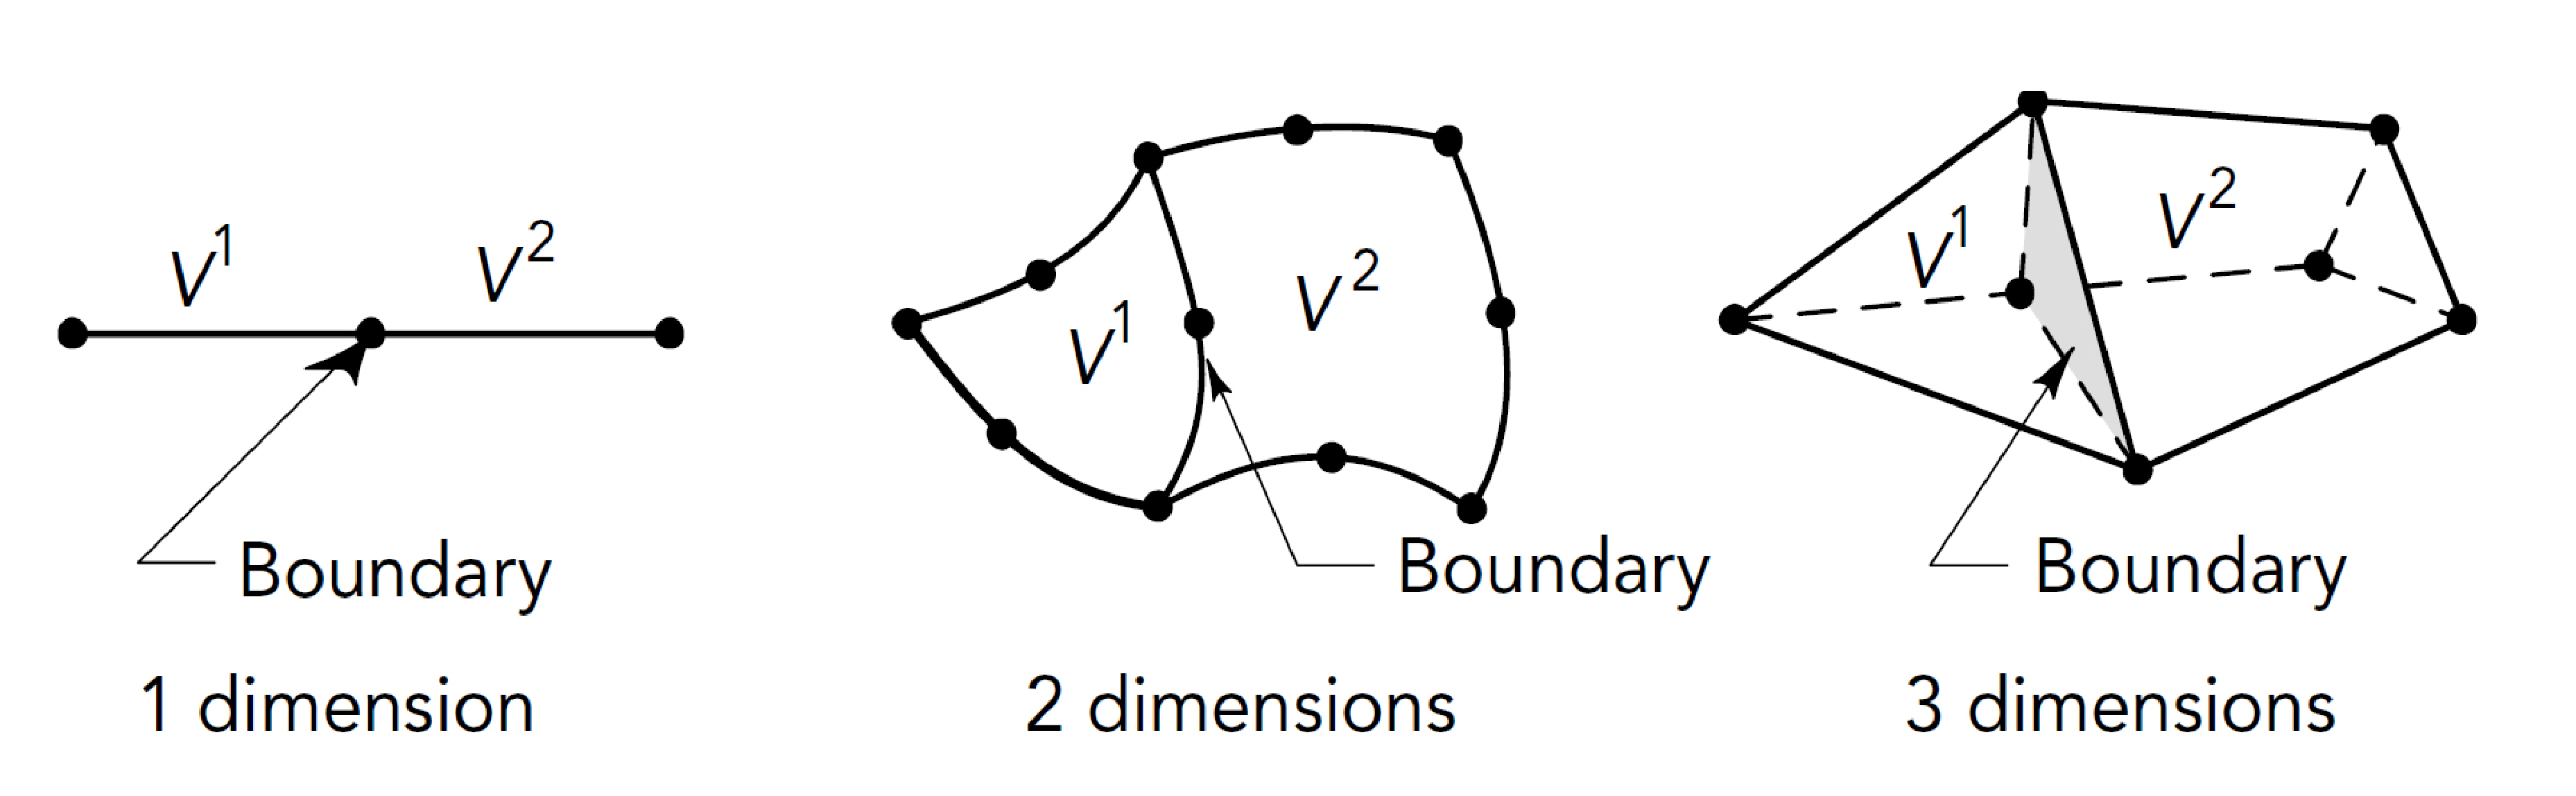
\includegraphics[scale=0.25]{../grafics/elements/exemples.pdf}
\caption{Exemples d'elements de diferents tipus i diferents dimensions. Tamb\'{e} es mostren les fronteres entre diversos elements. El primer exemple \'{e}s una divisi\'{o} d'un segment en dos elements, que tamb\'{e} s\'{o}n segments. Els nodes s\'{o}n els extrems dels elements. Al segon exemple hi ha un element triangular i un quadrangular. Tots dos tenen nodes no nom\'{e}s als v\`{e}rtexs, sin\'{o} que al mig de cada aresta tenen un altre node, que permet definir la curvatura de les fronteres. El tercer exemple consta d'un tetr\`{a}edre i un prisma triangular. Aquests tenen com a nodes nom\'{e}s els v\`{e}rtexs, de manera que les seves fronteres estan formades per segments. Font: \emph{Finite Element Method} \cite{dhatt2012finite}.}
\label{Fig:Exempleselements}
\end{center}
\end{figure}

Sobre cada element, la funci\'{o} $u(\boldsymbol{x})$ es posa com a combinaci\'{o} lineal d'unes certes funcions $P_1(\boldsymbol{x}),\ldots,P_n(\boldsymbol{x})$, de manera que tenim
\[u(\boldsymbol{x})=a_1P_1(\boldsymbol{x})+\cdots a_nP_n(\boldsymbol{x})\]
per uns certs coeficients $a_1,\ldots,a_n$. Per determinar aquests coeficients \'{e}s necessari i suficient con\`{e}ixer el valor exacte de $u_{\text{ex}}(x)$ o alguna de les seves derivades sobre $n$ punts $\boldsymbol{x}_1,\ldots,\boldsymbol{x}_n$ anomenats \textbf{nodes d'interpolaci\'{o}}, que acostumen a ser els mateixos que els nodes geom\`{e}trics, per\`{o} no tenen per qu\`{e}. D'aquesta manera estem transformant un problema de resoldre una equaci\'{o} diferencial en resoldre una mera equaci\'{o} algebraica.

Un cas particular molt utilitzat \'{e}s prendre com a coeficients els propis valors de la funci\'{o} $u_1=u_{\text{ex}}(\boldsymbol{x}_1),\ldots,u_n=u_{\text{ex}}(\boldsymbol{x}_n)$. D'aquesta manera queda
\[u(x)=u_1N_1(\boldsymbol{x})+\cdots+u_nN_n(\boldsymbol{x}),\]
per certes funcions $N_1(\boldsymbol{x}),\ldots,N_n(\boldsymbol{x})$ anomenades \textbf{funcions d'interpolaci\'{o}}.

Fixem-nos que aquestes funcions han de complir que $N_i(\boldsymbol{x}_i)=1$ i $N_i(\boldsymbol{x}_j)$ sempre que $i\neq j$. D'aquesta manera podem construir les nostres funcions $N_1(\boldsymbol{x}),\ldots,N_n(\boldsymbol{x})$ en funci\'{o} nom\'{e}s de la geometria dels elements i al marge de la funci\'{o} $u(\boldsymbol{x})$.
\vspace{5mm}

Normalment, per simplificar el problema, es treballa amb \textbf{elements de refer\`{e}ncia}, que s\'{o}n elements del mateix tipus que els que conformen la malla, per\`{o} amb posici\'{o}, orientaci\'{o} i forma molt m\'{e}s simple.

Aleshores, mitjan\c{c}ant una transformaci\'{o} $\boldsymbol{\tau}^e$, podem transformar l'element de refer\`{e}ncia $V^r$ en l'element $V^e$.
\[\boldsymbol{\tau}^e:\boldsymbol{\xi}\longrightarrow\boldsymbol{x}^e,\]
on $\boldsymbol{\xi}$ s\'{o}n els punts de $V^r$ i $\boldsymbol{x}^e$ s\'{o}n els punts de $V^e$. Voldrem que $\boldsymbol{\tau}^e$ sigui bijectiva, de manera que podem interpretar aquesta funci\'{o} com un canvi de coordenades des de les coordenades de refer\`{e}ncia a les coordenades de l'element real. Tamb\'{e} exigirem que envi\"{i} nodes de $V^r$ a nodes de $V^e$ i fronteres a fronteres.
\begin{figure}[ht!]
\begin{center}
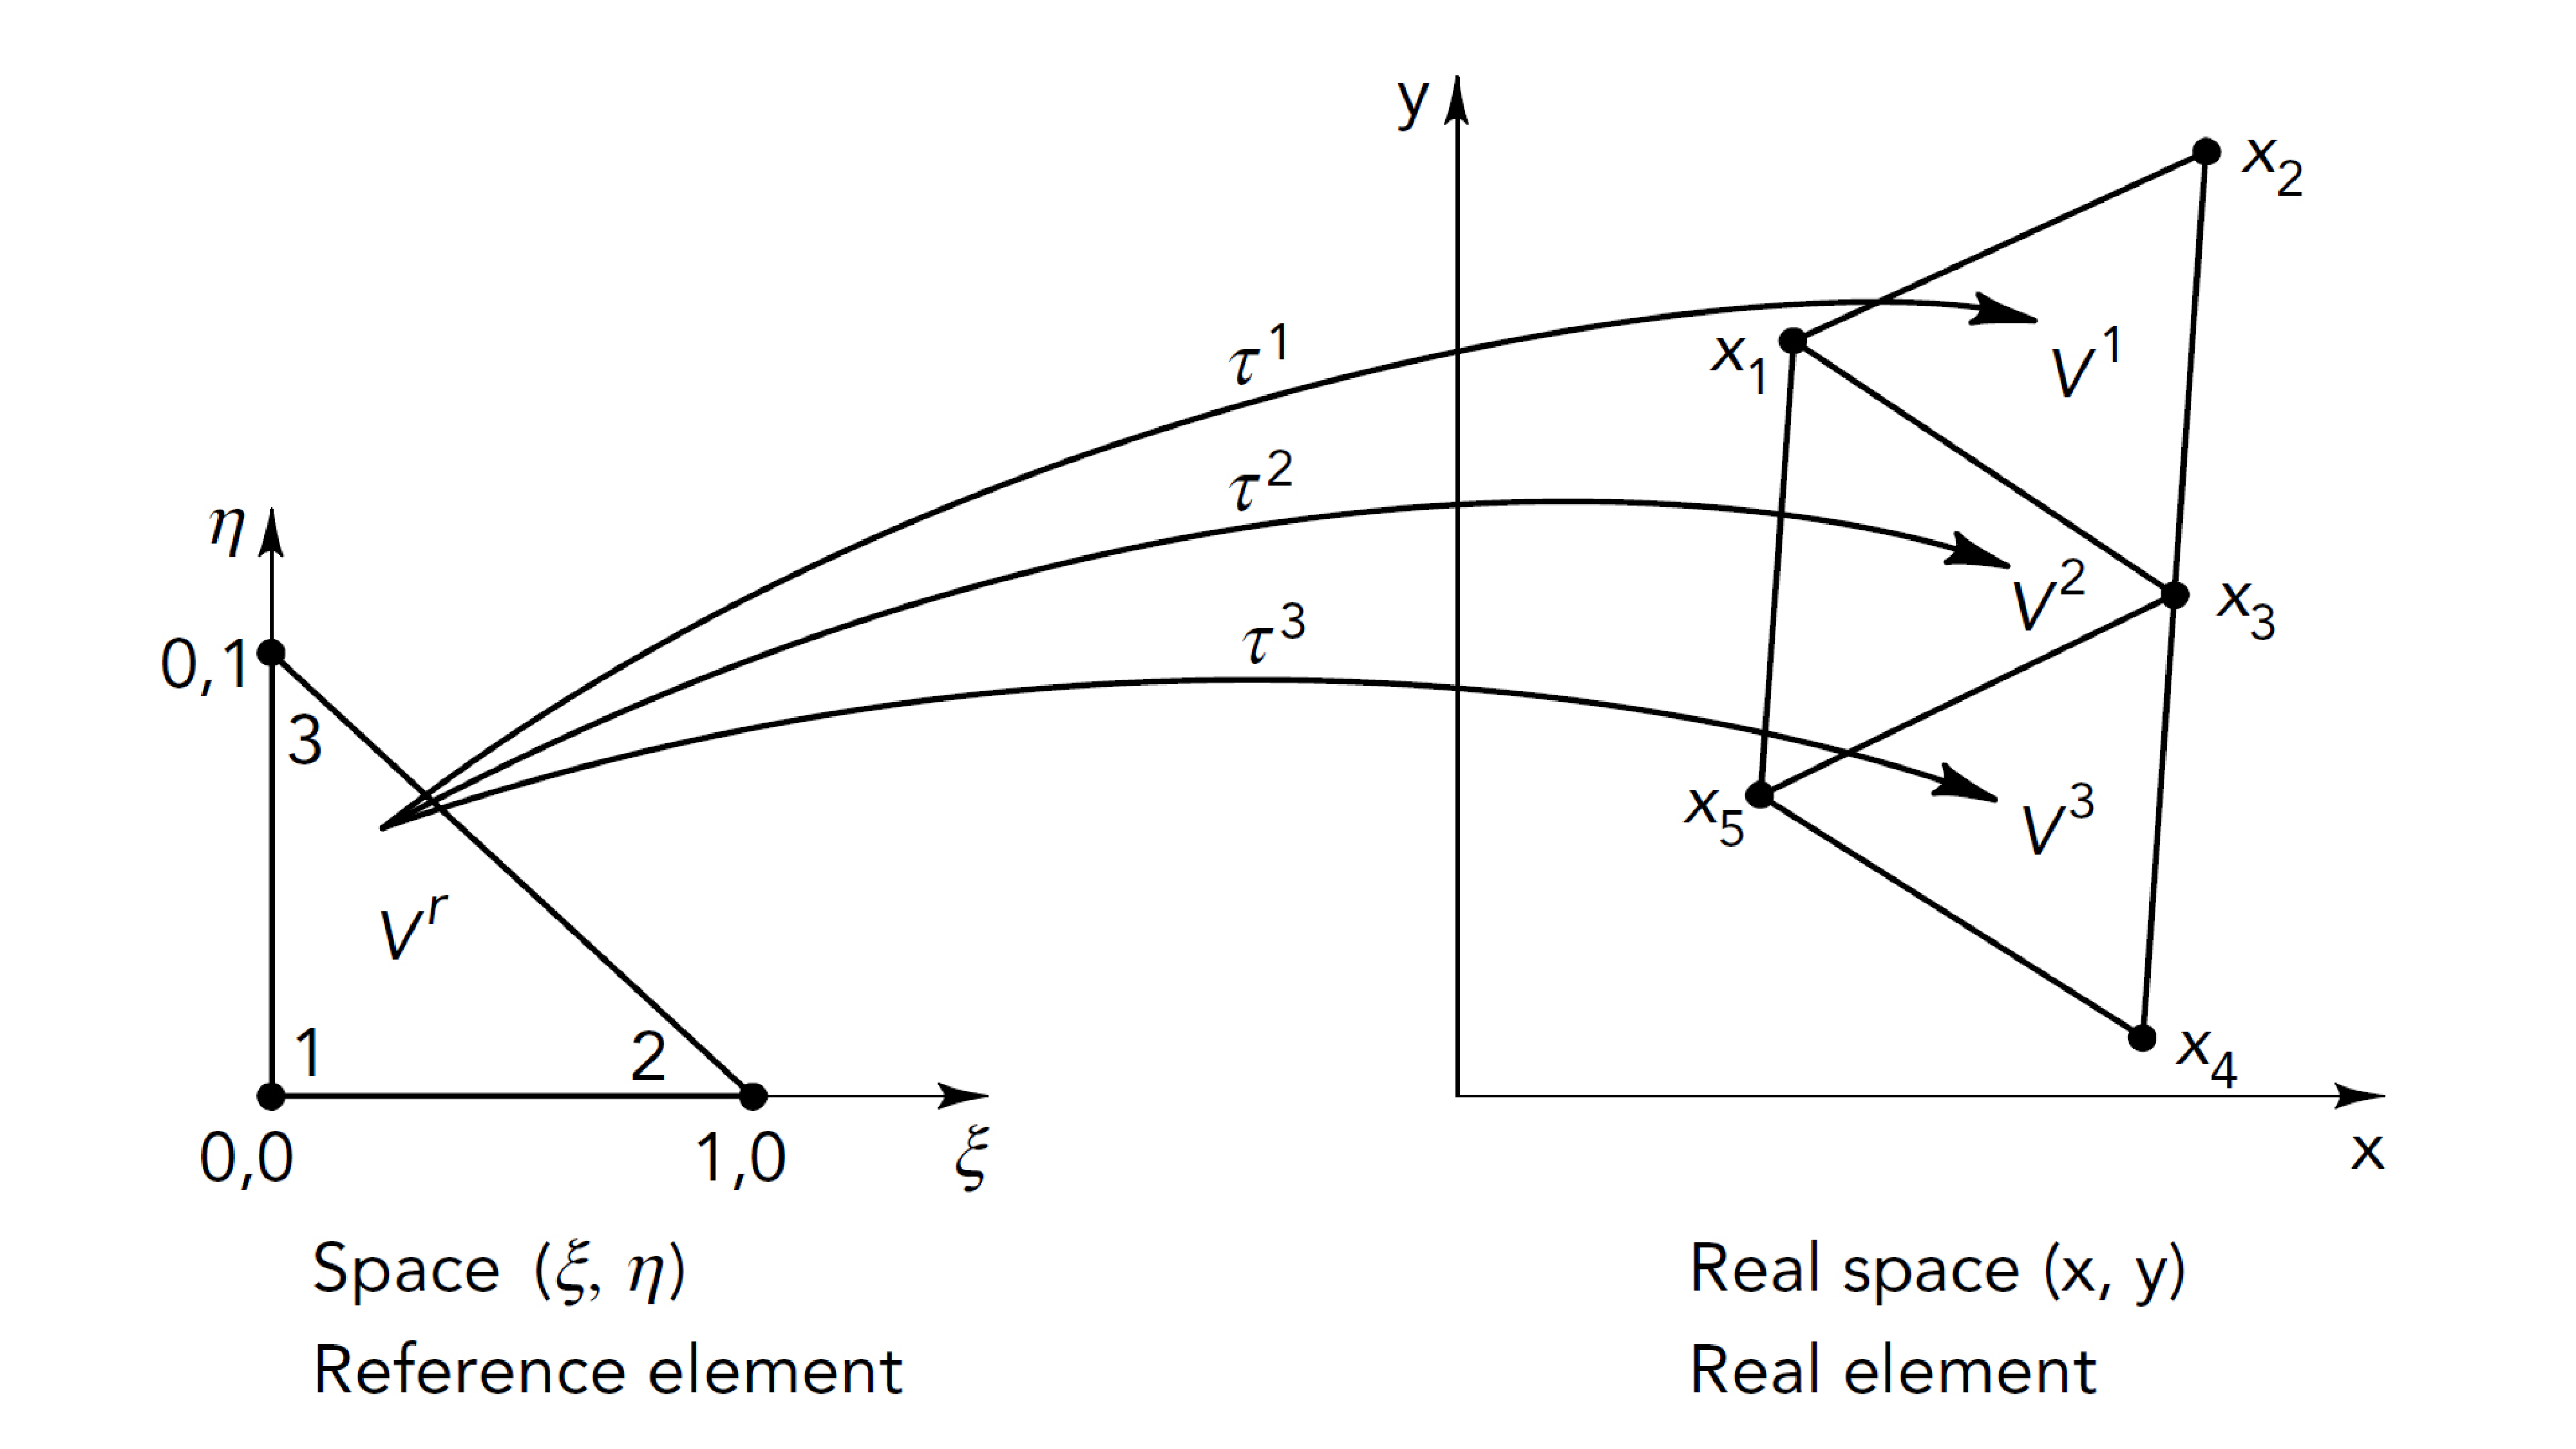
\includegraphics[scale=0.25]{../grafics/elements/transformacio.pdf}
\caption{Representaci\'{o} gr\`{a}fica de la transformaci\'{o} $\boldsymbol{\tau}$ amb l'exemple de triangles amb tres nodes. Font: \emph{Finite Element Method} \cite{dhatt2012finite}.}
\label{Fig:Transformaciotau}
\end{center}
\end{figure}

Cada $\boldsymbol{\tau}^e$ envia l'element de refer\`{e}ncia $V^r$ ---que \'{e}s sempre el mateix--- a cada element $V^e$. Per\`{o} hem dit que els elements estan enterament definits pels seus nodes. Per tant ha d'existir alguna funci\'{o} global $\boldsymbol{\tau}$ de manera que si $\boldsymbol{x}^e$ pertany a l'element definit pels nodes $\boldsymbol{x}_{i_1},\ldots,\boldsymbol{x}_{i_n}$, aleshores
\[\boldsymbol{\tau}(\boldsymbol{\xi};\boldsymbol{x}_{i_1},\ldots,\boldsymbol{x}_{i_n})=\boldsymbol{x}^e=\boldsymbol{\tau}^e(\boldsymbol{\xi}).\]

De fet, es pot trobar una $\boldsymbol{\tau}$ que sigui lineal en $\boldsymbol{x}_{i_1},\ldots,\boldsymbol{x}_{i_n}$. Encara podem anar m\'{e}s enll\`{a} i trobar una mateixa transformaci\'{o} per cada coordenada: existeix una aplicaci\'{o} lineal $\overline{N}(\boldsymbol{\xi})$ tal que si escrivim $\boldsymbol{x}^e=(x^e,y^e,z^e)$ i $\boldsymbol{x}_i=(x_i,y_i,z_i)$, aleshores
\begin{align*}
x^e(\boldsymbol{\xi})&=\overline{N}(\boldsymbol{\xi})(x_{i_1},\ldots,x_{i_n}),\\
y^e(\boldsymbol{\xi})&=\overline{N}(\boldsymbol{\xi})(y_{i_1},\ldots,y_{i_n}),\\
z^e(\boldsymbol{\xi})&=\overline{N}(\boldsymbol{\xi})(z_{i_1},\ldots,z_{i_n}).
\end{align*}
Si escrivim $\overline{N}(\boldsymbol{\xi})$ en forma matricial $\left(\begin{matrix}\overline{N}_1(\boldsymbol{\xi})&\cdots&\overline{N}_n(\boldsymbol{\xi})\end{matrix}\right)$, s'ent\'{e}n millor aquesta aplicaci\'{o}:
\begin{align*}
x^e(\boldsymbol{\xi})&=\overline{N}_1(\boldsymbol{\xi})\,x_{i_1}+\ldots+\overline{N}_n(\boldsymbol{\xi})\,x_{i_n},\\
y^e(\boldsymbol{\xi})&=\overline{N}_1(\boldsymbol{\xi})\,y_{i_1}+\ldots+\overline{N}_n(\boldsymbol{\xi})\,y_{i_n},\\
z^e(\boldsymbol{\xi})&=\overline{N}_1(\boldsymbol{\xi})\,z_{i_1}+\ldots+\overline{N}_n(\boldsymbol{\xi})\,z_{i_n}.
\end{align*}

D'aquestes expressions es dedueix que si $\boldsymbol{\xi}_j$ \'{e}s un node del domini de refer\`{e}ncia que va a parar al node $\boldsymbol{x}_{i_j}$, aleshores s'ha de complir que $\overline{N}_j(\boldsymbol{\xi}_j)=1$ i que $\overline{N}_k(\boldsymbol{\xi}_j)=0$ per tot $k\neq j$. Per tant les funcions $\overline{N}_j(\boldsymbol{\xi})$ es construeixen com funcions escalars sobre el domini de refer\`{e}ncia que valen 1 al node $\boldsymbol{\xi}_j$ i 0 a la resta de nodes. Aquestes funcions s'acostumen a dir \textbf{funcions geom\`{e}triques de transformaci\'{o}} i normalment triem funcions $\overline{N}(\boldsymbol{\xi})$ que siguin polinomials per $\boldsymbol{\xi}$. Ens fixem que les funcions geom\`{e}triques de transformaci\'{o} s\'{o}n an\`{a}logues a les funcions d'interpolaci\'{o} anteriorment esmentades. De fet, en el cas que els nodes d'interpolaci\'{o} i els nodes geom\`{e}trics coincideixen, les funcions $N_j(\boldsymbol{x})$ i $\overline{N}_j(\boldsymbol{\xi})$ s\'{o}n la mateixa funci\'{o}, tret que una est\`{a} expressada a l'espai dels elements reals i l'altra a l'espai de l'element de refer\`{e}ncia.

Exemplifiquem aquestes transformacions $\boldsymbol{\tau}$ i $\overline{N}$ amb elements triangulars. Podem considerar el triangle de la Figura \ref{Fig:Transformaciotau}, de v\`{e}rtexs $(0,0)$, $(1,0)$ i $(0,1)$. Si escrivim les coordenades com $\boldsymbol{\xi}=(\xi,\eta)$, aleshores l'element de refer\`{e}ncia \'{e}s el que compleix les desigualtats
\begin{align*}
\xi+\eta&\leq1,\\
\xi&\geq0,\\
\eta&\geq0.
\end{align*}

Volem transformar aquest triangle en un triangle de v\`{e}rtexs $\boldsymbol{x}_i=(x_i,y_i),\boldsymbol{x}_j=(x_j,y_j),\boldsymbol{x}_k=(x_k,y_k)$. Volem trobar la transformaci\'{o} $\boldsymbol{\tau}$ que va del triangle de refer\`{e}ncia a aquest triangle general. Per all\`{o} busquem les aplicacions $\overline{N}_1(\xi,\eta),\overline{N}_2(\xi,\eta),\overline{N}_3(\xi,\eta)$, les quals hem dit que no depenen de $\boldsymbol{x}_i,\boldsymbol{x}_j,\boldsymbol{x}_k$, sin\'{o} nom\'{e}s del triangle de refer\`{e}ncia. Buscarem funcions afins, ja que s\'{o}n les m\'{e}s senzilles.

L'aplicaci\'{o} $\overline{N}_1(\xi,\eta)$ ha de valer 1 al $(0,0)$ i 0 al $(1,0)$ i al $(0,1)$. Per tant proposem $N_1(\xi,\eta)=1-\xi-\eta$. L'aplicaci\'{o} $\overline{N}_2(\xi,\eta)$ ha de valer 1 al $(1,0)$ i 0 al $(0,0)$ i al $(0,1)$. Per tant proposem $N_2(\xi,\eta)=\xi$. Seguint el mateix raonament, tenim $N_3(\xi,\eta)=\eta$. En total, la transformaci\'{o} resultant \'{e}s:
\[x(\xi,\eta)=\left(\begin{matrix}1-\xi-\eta&\xi&\eta\end{matrix}\right)\left(\begin{matrix}x_i\\x_j\\x_k\end{matrix}\right),\hspace{7mm}y(\xi,\eta)=\left(\begin{matrix}1-\xi-\eta&\xi&\eta\end{matrix}\right)\left(\begin{matrix}y_i\\y_j\\y_k\end{matrix}\right).\]

Es pot comprovar que efectivament aquesta transformaci\'{o} fa correspondre el triangle de refer\`{e}ncia que hem posat amb el triangle format pels v\`{e}rtexs $\boldsymbol{x}_i,\boldsymbol{x}_j,\boldsymbol{x}_k$; a m\'{e}s que fa correspondre els nodes $(0,0)$, $(1,0)$, $(0,1)$ als nodes $\boldsymbol{x}_i,\boldsymbol{x}_j,\boldsymbol{x}_k$ respectivament i els costats als costats corresponents. A m\'{e}s, es pot comprovar f\`{a}cilment que la transformaci\'{o} \'{e}s bijectiva.
\vspace{5mm}

Aix\`{o} de treballar amb elements de refer\`{e}ncia ho hem presentat perqu\`{e} \'{e}s molt m\'{e}s f\`{a}cil treballar sobre l'espai de les $\boldsymbol{\xi}$ que sobre l'espai de les $\boldsymbol{x}$, ja que hem pres la refer\`{e}ncia perqu\`{e} sigui especialment simple. D'aquesta manera, passem a expressar la funci\'{o} $\boldsymbol{u}(\boldsymbol{x})=\boldsymbol{u}(\boldsymbol{\tau}(\boldsymbol{\xi}))$ sobre les coordenades $\boldsymbol{\xi}$. Per simplicitat escriurem simplement $\boldsymbol{u}(\boldsymbol{\xi})=\boldsymbol{u}(\boldsymbol{x})$. Aix\'{i}, escriurem
\[u(\boldsymbol{\xi})=u_1N_1(\boldsymbol{\xi})+\cdots+u_nN_n(\boldsymbol{\xi}).\]
Recordem que si coincideixen els nodes d'interpolaci\'{o} i els nodes geom\`{e}trics, aleshores $N_i(\boldsymbol{\xi})=\overline{N}_i(\boldsymbol{\xi})$.

Quan prenem les coordenades de $\boldsymbol{\xi}$, avaluar la funci\'{o} \'{e}s directe: $u(\boldsymbol{\xi})=u_1N_1(\boldsymbol{\xi})+\cdots+u_nN_n(\boldsymbol{\xi})$, per\`{o} si hem d'avaluar les derivades parcials, hem de fer servir la regla de la cadena, que permet escriure les derivades respecte les coordenades de $\boldsymbol{x}$ en termes de derivades respecte les coordenades de $\boldsymbol{\xi}$. Aix\'{i}, si anomenem les coordenades de $\boldsymbol{\xi}$ com $\xi,\eta,\zeta$, tenim
\[\left(\begin{matrix}\displaystyle{\frac\partial{\partial x}}\vspace{1mm}\\\displaystyle{\frac\partial{\partial y}}\vspace{1mm}\\\displaystyle{\frac\partial{\partial z}}\end{matrix}\right)=\left(\begin{matrix}\displaystyle{\frac{\partial\xi}{\partial x}}&\displaystyle{\frac{\partial\eta}{\partial x}}&\displaystyle{\frac{\partial\zeta}{\partial x}}\vspace{1mm}\\\displaystyle{\frac{\partial\xi}{\partial y}}&\displaystyle{\frac{\partial\eta}{\partial y}}&\displaystyle{\frac{\partial\zeta}{\partial y}}\vspace{1mm}\\\displaystyle{\frac{\partial\xi}{\partial z}}&\displaystyle{\frac{\partial\eta}{\partial z}}&\displaystyle{\frac{\partial\zeta}{\partial z}}\end{matrix}\right)\left(\begin{matrix}\displaystyle{\frac\partial{\partial\xi}}\vspace{1mm}\\\displaystyle{\frac\partial{\partial\eta}}\vspace{1mm}\\\displaystyle{\frac\partial{\partial\zeta}}\end{matrix}\right).\]

Aquesta igualtat matricial es pot escriure de forma compacta com $(\partial\boldsymbol{x})=j(\partial\boldsymbol{\xi})$. La matriu $j$ \'{e}s la matriu jacobiana del canvi de coordenades $\boldsymbol{\tau}^{-1}$, per\`{o}, tret dels casos m\'{e}s simples, no ser\`{a} gens f\`{a}cil invertir l'aplicaci\'{o} $\boldsymbol{\tau}$. Per aix\`{o}, si $J$ \'{e}s la jacobiana de $\boldsymbol{\tau}$, que es pot calcular perfectament, aleshores podem obtenir $j$ com $j=J^{-1}$; \'{e}s a dir, nom\'{e}s ens cal invertir una matriu i no l'aplicaci\'{o} sencera. Gr\`{a}cies a aix\`{o}, ja podem posar la funci\'{o} $u_1N_1(\boldsymbol{\xi})+\cdots+u_nN_n(\boldsymbol{\xi})$ dins una equaci\'{o} diferencial de primer ordre i avaluar als nodes per obtenir aix\'{i} els coeficients $u_1,\ldots,u_n$. Si l'equaci\'{o} diferencial \'{e}s de segon ordre o superior, aleshores utilitzant la regla de la cadena d'ordres superiors, es poden trobar els coeficients igualment.

Recordem que al principi d'aquest ap\`{e}ndix hem dit: <<tant les funcions $u^e(\boldsymbol{x})$ com les seves derivades parcials han de ser compatibles a les fronteres comuns de dos subdominis per tal que la funci\'{o} total $u(\boldsymbol{x})$ sigui prou derivable>>. Volem que a la frontera com\'{u} de dos subdominis $V^{e_1}$ i $V^{e_2}$, les funcions $u^{e_1}(\boldsymbol{x})$ i $u^{e_2}(\boldsymbol{x})$, aix\'{i} com les seves derivades fins un cert ordre, prenguin els mateixos valors. Aix\`{o} ho aconseguim tenint que els $u^e(\boldsymbol{x})$, sobre els punts d'una frontera, depenguin nom\'{e}s dels nodes que defineixen aquella frontera. Aleshores, si volem que la funci\'{o} total $u(\boldsymbol{x})$ sigui cont\'{i}nua, n'hi ha prou amb exigir que cada funci\'{o} $N_i(\boldsymbol{\xi})$ valgui 0 sobre aquelles fronteres sobre les quals no hi estigui el node $\boldsymbol{\xi}_i$. D'igual manera, si volem que $u(\boldsymbol{x})$ sigui de classe $C^r$, imposem la mateixa condici\'{o}, per\`{o} sobre les derivades de $N_i(\boldsymbol{\xi})$ fins ordre $r$.

Un aspecte important del m\`{e}tode dels elements finits \'{e}s que la funci\'{o} $u(\boldsymbol{x})$ convergeixi a la funci\'{o} exacta $u_{\text{ex}}(\boldsymbol{x})$ quan la quantitat de nodes presos tendeix cap a infinit. Una condici\'{o} suficient que garanteix que l'error $u(\boldsymbol{x})-u_{\text{ex}}(\boldsymbol{x})$ tendeix cap a zero \'{e}s que a l'expressi\'{o} de $u(\boldsymbol{x})$ hi aparegui un terme constant. Aquesta condici\'{o} \'{e}s equivalent a que $u(\boldsymbol{x})$ coincideixi amb $u_{\text{ex}}(\boldsymbol{x})$ en el cas que la funci\'{o} a aproximar $u_{\text{ex}}(\boldsymbol{x})$ sigui constant. D'igual manera, una condici\'{o} suficient perqu\`{e} l'error de les derivades parcials fins ordre $r$ tendeixi cap a 0 \'{e}s que l'expressi\'{o} de $u(\boldsymbol{x})$ contingui un polinomi sencer d'ordre $r$ i aix\`{o} \'{e}s novament equivalent a que $u(\boldsymbol{x})$ sigui capa\c{c} d'aproximar amb total exactitud polinomis de grau m\'{e}s petit o igual que $r$.

Per calcular els coeficients $u_1,\ldots,u_n$ de l'expressi\'{o} $u(\boldsymbol{x})=u_1N_1(\boldsymbol{x})+\cdots+u_nN_n(\boldsymbol{x})$, la manera m\'{e}s senzilla \'{e}s substituir aquesta expressi\'{o} a l'equaci\'{o} diferencial i avaluar-la als nodes d'interpolaci\'{o} per aix\'{i} transformar l'equaci\'{o} diferencial en una equaci\'{o} algebraica d'inc\`{o}gnites $u_1,\ldots u_n$. De totes maneres, hi ha altres formes d'obtenir aquests coeficients. Una d'elles, que \'{e}s la que s'utilitza per l'equaci\'{o} hidrodin\`{a}mica, consisteix a multiplicar l'equaci\'{o} diferencial per la funci\'{o} $N_i(\boldsymbol{x})$ i integrar sobre el volum de l'element. Aix\`{o}, en llenguatge d'espais de Hilbert, \'{e}s projectar l'equaci\'{o} sobre els elements de la base que formen les funcions $N_1(\boldsymbol{x}),\ldots,N_n(\boldsymbol{x})$. Aix\'{i} s'obt\'{e} una equaci\'{o} algebraica sobre els coeficients. Aquest procediment es realitza per cadascuna de les $n$ funcions $N_i(\boldsymbol{x})$, obtenint-se aix\'{i} les $n$ equacions algebraiques a resoldre i que donen els valors dels coeficients $u_1,\ldots,u_n$.

\bibliographystyle{ieeetr}
\bibliography{bibliografia.bib}

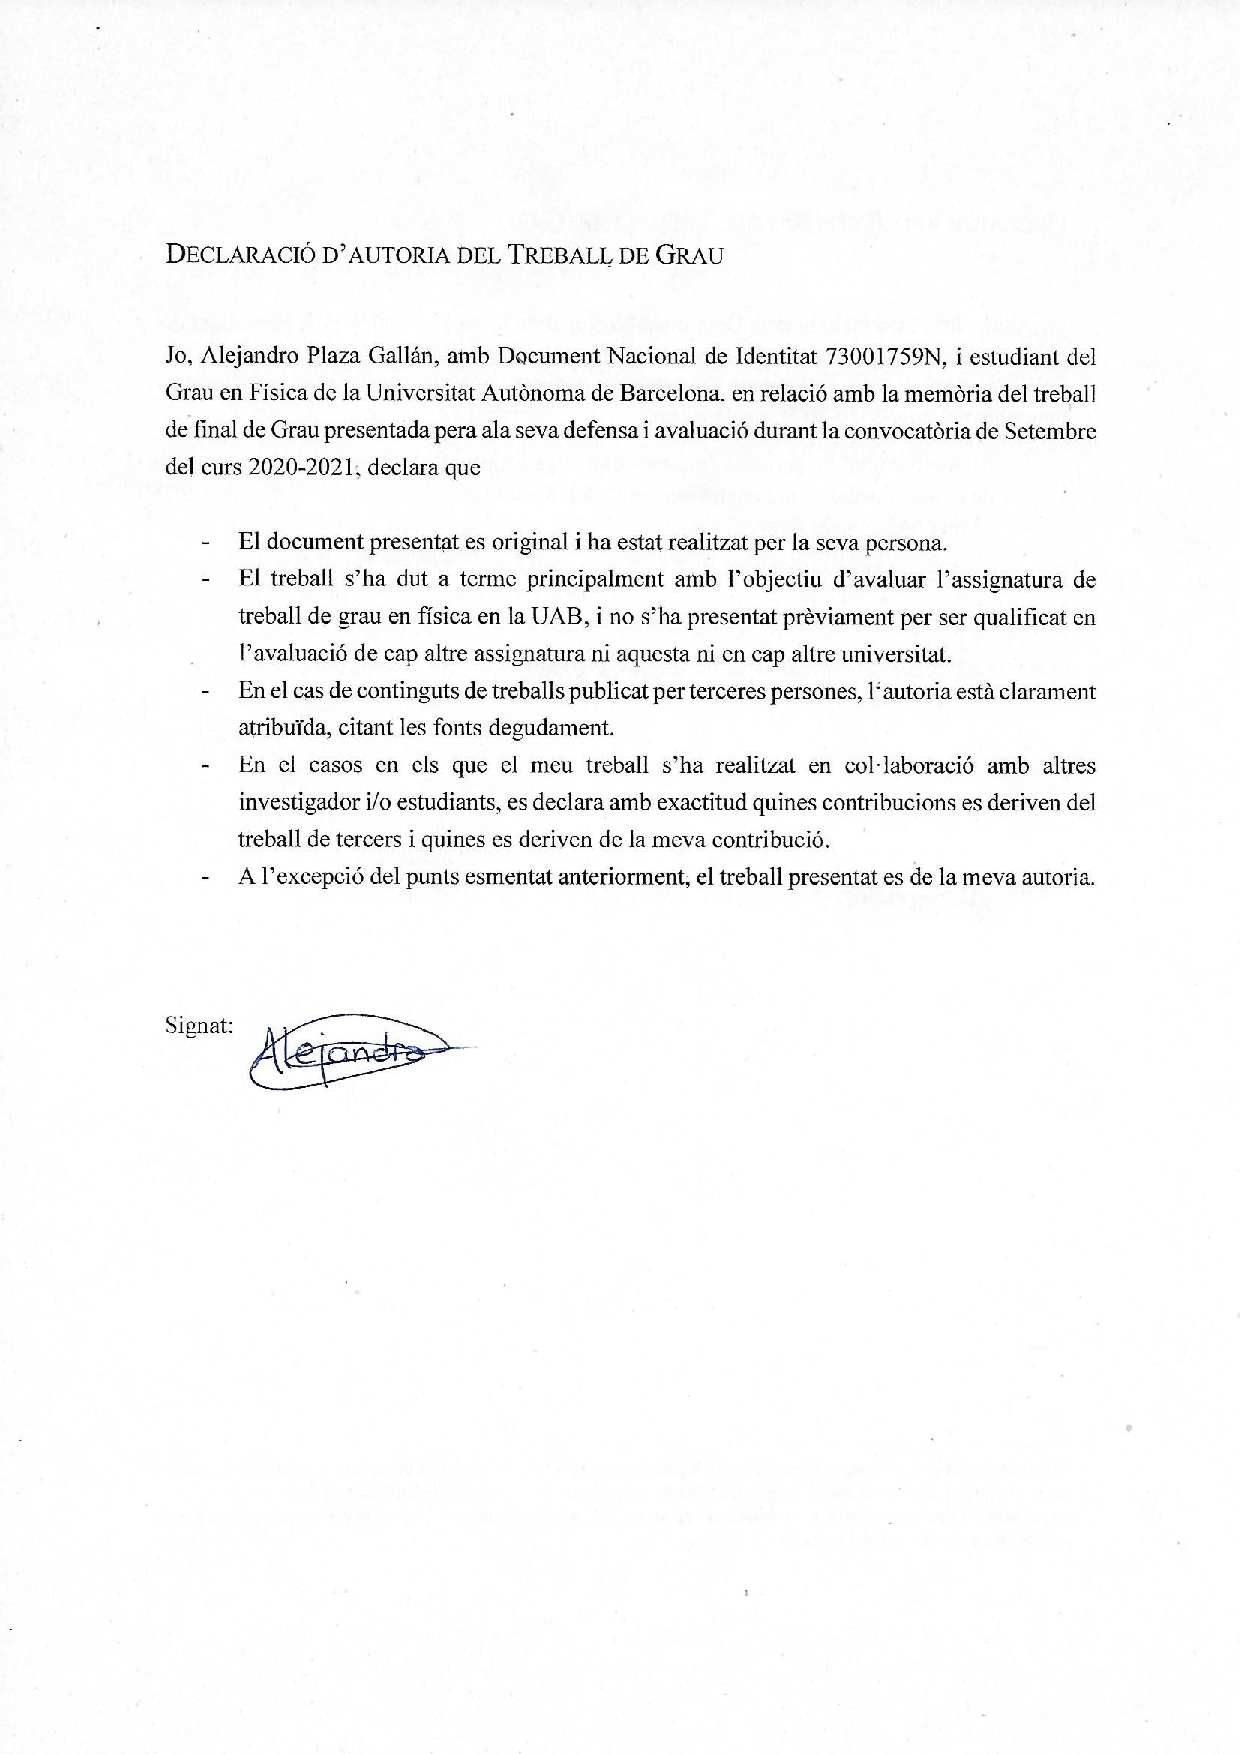
\includepdf[pages=-]{declaracio-dautoria.pdf}
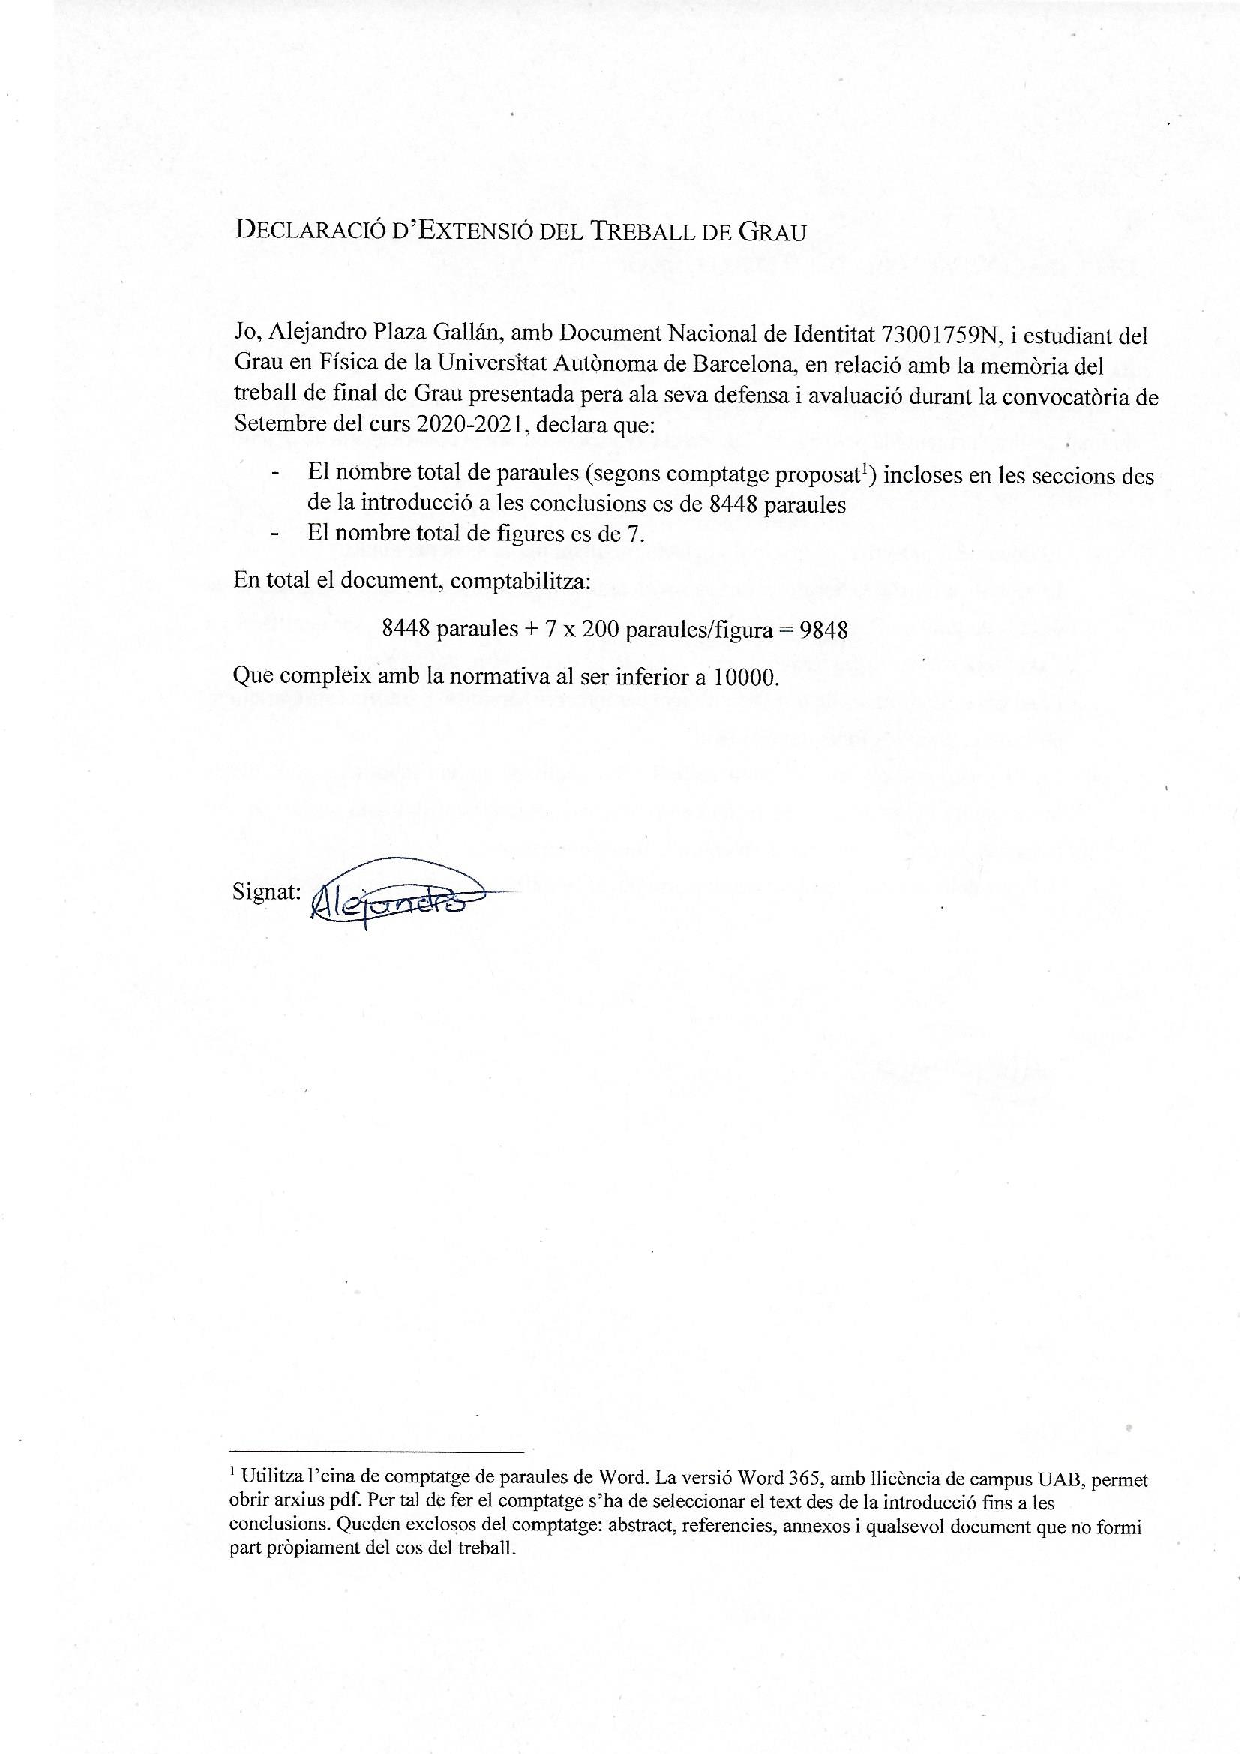
\includepdf[pages=-]{declaracio-dextensio.pdf}

\end{document}
